% Build: latexmk -pdf -interaction=nonstopmode -halt-on-error prism.tex
% Self-contained article. All displayed Prism syntax is a design specification.
\documentclass[11pt,a4paper]{article}
\usepackage[T1]{fontenc}
\usepackage[utf8]{inputenc}
\usepackage{lmodern,microtype}
\usepackage[margin=24mm,headheight=15pt]{geometry}
\usepackage{amsmath,amssymb,amsthm,mathtools,stmaryrd}
\SetSymbolFont{stmry}{bold}{U}{stmry}{m}{n}
\usepackage{booktabs,tabularx,longtable,array}
\usepackage{xcolor,listings,enumitem,fancyhdr,titlesec,needspace,etoolbox}
\usepackage{tikz}
\usetikzlibrary{arrows.meta,positioning}
\usepackage{xurl}
\usepackage[colorlinks=true,linkcolor=teal!55!black,citecolor=teal!55!black,urlcolor=teal!55!black]{hyperref}
\usepackage{bookmark}
\definecolor{ink}{HTML}{283E3B}
\definecolor{accent}{HTML}{386D66}
\definecolor{panel}{HTML}{F2F5F3}
\definecolor{muted}{HTML}{586560}
\definecolor{rulegray}{HTML}{CAD4CF}
\titleformat{\section}{\Large\sffamily\bfseries\color{ink}}{\thesection}{.65em}{}
\titleformat{\subsection}{\large\sffamily\bfseries\color{ink}}{\thesubsection}{.65em}{}
\titleformat{\subsubsection}{\normalsize\bfseries\color{ink}}{\thesubsubsection}{.6em}{}
\setlength{\parindent}{0pt}
\setlength{\parskip}{.42em}
\setlength{\emergencystretch}{2em}
\setcounter{tocdepth}{1}
\setlist{nosep,leftmargin=1.5em}
\renewcommand{\arraystretch}{1.15}
\newcolumntype{Y}{>{\raggedright\arraybackslash}X}
\newcolumntype{P}[1]{>{\raggedright\arraybackslash}p{#1}}
\pagestyle{fancy}
\fancyhf{}
\fancyhead[L]{\small\sffamily Prism: proof language and certified computation}
\fancyhead[R]{\small\sffamily Second iteration}
\fancyfoot[C]{\small\thepage}
\renewcommand{\headrulewidth}{.3pt}
\lstdefinestyle{prism}{basicstyle=\small\ttfamily,columns=fullflexible,
 keepspaces=true,breaklines=true,breakatwhitespace=false,showstringspaces=false,
 backgroundcolor=\color{panel},frame=single,rulecolor=\color{rulegray},
 framerule=.3pt,framesep=6pt,xleftmargin=6pt,xrightmargin=6pt,
 aboveskip=.8em,belowskip=.6em,tabsize=2}
\lstset{style=prism}
\newcommand{\code}[1]{\texttt{\detokenize{#1}}}
\newcommand{\N}{\mathbb N}
\newcommand{\Z}{\mathbb Z}
\newcommand{\Q}{\mathbb Q}
\newcommand{\R}{\mathbb R}
\newcommand{\C}{\mathbb C}
\newcommand{\Rep}{\operatorname{Rep}}
\newcommand{\Claim}{\operatorname{Claim}}
\newcommand{\coeff}[2]{[#1]#2}
\newcommand{\ord}{\operatorname{ord}}
\newcommand{\E}{\mathcal E}
\newcommand{\G}{\Gamma}
\newcommand{\prism}{\textsc{Prism}}
\newtheorem{proposition}{Proposition}[section]
\newtheorem{lemma}[proposition]{Lemma}
\newtheorem{theorem}[proposition]{Theorem}
\theoremstyle{definition}
\newtheorem{definition}[proposition]{Definition}
\theoremstyle{remark}
\newtheorem{remark}[proposition]{Remark}
\hypersetup{pdftitle={Prism: A Proof Language with Certified Mathematical Computation},
 pdfauthor={OpenAI, for Vladimir Reshetnikov},
 pdfsubject={Second-iteration proof-language design grounded in Brainstorm, ProveIt, and Leant},
 bookmarksnumbered=true}
\pretocmd{\section}{\Needspace{7\baselineskip}}{}{}
\pretocmd{\subsection}{\Needspace{4\baselineskip}}{}{}
\begin{document}
\begin{titlepage}
\vspace*{10mm}
{\sffamily\small\color{muted}BRAINSTORM / SECOND ITERATION / TECHNICAL DESIGN STUDY\par}
\vspace{14mm}
{\sffamily\bfseries\color{ink}\fontsize{32}{38}\selectfont Prism\par}
\vspace{4mm}
{\sffamily\bfseries\color{ink}\fontsize{23}{29}\selectfont A Proof Language with\\Certified Mathematical Computation\par}
\vspace{9mm}
{\sffamily\Large Mathematical objects, explicit choices,\\and checkable changes of representation\par}
\vspace{12mm}
\begin{quote}
\large A symbolic computation should not merely return an expression. It should return an expression \emph{together with the exact mathematical relationship it has to the input}.
\end{quote}
\vspace{8mm}
This proposal takes the two Brainstorm syntheses as its starting point, rather than proposing another vocabulary for the same architecture. It develops their less resolved boundary: how a concise proof language can support definitions, multiple mathematical representations, symbolic algorithms, and rigorous numerical information within one Lean-checked document.
\vfill
{\sffamily Prepared for Vladimir Reshetnikov\par}
{\sffamily OpenAI\par}
{\sffamily 5 September 2026, Pacific time\par}
\vspace{5mm}
{\small\color{muted}\textbf{Evidence status.} The article contains a proposed language and architecture, paper proofs of its mathematical contracts, static repository inspection, and executed exact-arithmetic experiments. It does not contain an implemented Prism compiler or a Lean-checked formalization of the new contracts. Proposed syntax is illustrative, not an assertion that it currently compiles.\par}
\end{titlepage}

\begin{abstract}
The first Brainstorm iteration converged on a sensible architecture: Lean-hosted mathematical steps, fixed statements, scoped obligations, ordinary theorem-backed methods, honest synthesis outcomes, and retained evidence. Repeating that consensus would contribute little. This article proposes a specific extension: an object-centered mathematical workbench in which \emph{certified computations and certified changes of representation are first-class proof steps}. The central interface is relational. Exact equality, equality on a domain, equality of germs, equivalence of solution sets, agreement of finite series coefficients, and numerical enclosure are different claims with different composition rules. A computer algebra system may optimize the representation of a fixed mathematical object, but may not silently change the object, its domain, or the strength of the claim.

The design combines theorem-annotated methods with verified computational kernels and independently checked certificates. It gives explicit rules for dependent guard composition, directional abstraction, and precision propagation. Worked developments cover binomial inversion over additive commutative groups, autonomous derivatives with a symbolic Lambert-type polynomial recurrence, Abel-series coefficients over arbitrary commutative rational algebras, and an exact root enclosure. A small executable companion checks 2,475 finite arithmetic instances and mutation tests; its limited evidential role is stated precisely. The implementation proposal reuses Lean and Leant, starts with a compact polynomial-certificate path, and compares ordinary Lean and a mathematical frontend over identical libraries. Success is reduced mathematical bookkeeping and better reading and repair, not a new syntax at any cost.
\end{abstract}
\begingroup
\small
\setlength{\parskip}{0pt}
\makeatletter
\renewcommand*\l@section{\@dottedtocline{1}{0em}{2em}}
\makeatother
\tableofcontents
\endgroup
\clearpage

\section{What should change in the second iteration?}\label{sec:second}
\subsection{The inherited architecture is a baseline, not the new idea}
The two supplied syntheses have different emphases. \emph{Mathematical Ideas, Checked Evidence} develops the common contract, reviews Leant's candidate and suggestion boundaries, and proposes a two-frontend experiment. \emph{Nine Blueprints for a Mathematician's Proof Language over Lean} adds a broad lexical corpus audit, argues for methods as annotated theorem types, and asks whether definitions are a larger source of friction than proof syntax. Both eventually accept important qualifications about corpus measurements, statement notices, and tactic-text replay~\cite{synA,synB}.

I retain their shared foundation: use Lean as the first logical host; keep mathematical choices visible; certify every formal assertion, including unused ones; distinguish accepted objects from proofs about them; and retain evidence instead of repeatedly rediscovering it. I also retain their experimental discipline. The new frontend must be compared with ordinary Lean supplied with the \emph{same} helper theorems, normalizers, and synthesis services.

My departure is to make the central artifact slightly richer than an obligation ledger. A ledger answers, ``What must still be proved?'' A mathematical workbench should also answer:
\begin{quote}
What object are we studying, which representation are we using, what operation are we asking for, and what exactly will its answer establish?
\end{quote}
That question connects the proof layer to the CAS layer and, importantly, to the definition layer. It is the organizing principle of \prism. The name is only a local label for this proposal.

\subsection{Five concrete design decisions}
\begin{enumerate}
\item \textbf{Representations are anchored to mathematical objects.} A sparse polynomial, a formal series, and a coefficient oracle may describe related mathematics, but each relationship is certified. Replacing a representation is not permission to replace an arbitrary chosen object.
\item \textbf{Computations return typed mathematical claims.} ``Simplify,'' ``solve,'' ``differentiate,'' and ``approximate'' have distinct result contracts. Their outputs are not all equations.
\item \textbf{Guards and precision compose with the computation.} A denominator condition, a local domain, or an available series order is part of the operation's interface. It cannot disappear when intermediate expressions are hidden.
\item \textbf{The CAS has two evidence paths.} Small kernels are verified algorithms; larger search procedures may be untrusted certificate producers. Both paths end in Lean-checkable claims about the original objects.
\item \textbf{Definitions get interfaces before they get new prose syntax.} Begin with representation packages and proved interface lemmas, not a general-purpose natural-language definition parser.
\end{enumerate}
These decisions refine ideas already present in the syntheses. They are not claims that relational transfer, proof-producing algebra, or verified numerics were invented here.

\subsection{What this proposal deliberately does not promise}
There is no universal simplifier, complete solver for arbitrary mathematics, automatic recognition of every intended convention, or proof that a displayed explanation matches a human's mental process. An unsuccessful computation leaves a precise request unsolved. A useful partial answer may still be returned, but its weaker contract remains visible.

Nor is a successful Lean proof automatically evidence that the \emph{language} helped. For example, the current binomial-inversion development already factors its main mathematics through a lower-triangular-kernel API~\cite{binomial}. Its compact public results are controls against unnecessary redesign, not opportunities to claim dramatic compression by hiding an existing theorem call.

\section{Evidence from the repositories}\label{sec:source}
\subsection{Inspected snapshots and limits}
The following are the public revisions resolved during this study. They differ from some local working-tree snapshots discussed inside the syntheses. In particular, the syntheses' uncommitted Leant extensions are not treated here as features verified in the public revision.
\begin{center}\small
\begin{tabularx}{\textwidth}{@{}l l Y@{}}
\toprule
Repository & Revision prefix & Direct inspection used here\\
\midrule
Brainstorm & \code{494be9d5ab41} & Both synthesis texts, including their questions for the next round.\\
ProveIt & \code{24ce8bd743ea} & BinomialInversion, AutonomousIteratedDeriv, AbelPolynomialSeries.\\
Leant & \code{3a40904be8a4} & Verification module, Engine boundary and origin types, selected Main suggestion code.\\
\bottomrule
\end{tabularx}
\end{center}
Full commit identifiers and paths are recorded in the bibliography and companion source register. The inspection was static. No ProveIt or Leant build was run. Individual first-round proposals are discussed through the two syntheses unless explicitly identified otherwise; this is not a second independent audit of all nine originals.

\subsection{Binomial inversion: representations obscure a short argument}
The kernel identity is
\begin{equation}\label{eq:orth}
\sum_{k=j}^{n}(-1)^{n-k}\binom nk\binom kj=[n=j],
\end{equation}
with the sum interpreted as empty for $n<j$. The inspected proof contains exactly the expected mathematics: remove the empty case, write $n=j+m$, reindex by $k=j+i$, apply the binomial product identity, and use the alternating binomial sum. Around those choices are interval-to-range conversion, arithmetic equalities about natural subtraction, cast transport, and ring normalization~\cite{binomial}.

The lesson is not simply that Lean requires too many lines. The author alternates between several interfaces to the \emph{same finite calculation}. A better interface should let the author select the index map and the identity, then recover the index and scalar transports from that context. Crucially, the module-valued theorem holds for an arbitrary additive commutative group. A CAS defaulting to rational vector spaces would silently weaken the result.

\subsection{Autonomous derivatives: locality is part of the proof}
The inspected theorem establishes
\[
W^{(n)}(x)=G_n(W(x))\qquad(x\in U)
\]
from an autonomous derivative equation and a recurrence for $G_n$. Its hypotheses require the derivative of $G_n$ only at values reached by $W$ on $U$. In the successor step the source constructs eventual equality near $x$ using openness of $U$, transfers the derivative, and applies the chain rule~\cite{ode}.

There are two different tasks here. Establishing neighborhood equality belongs to mathematical reasoning about the context. Differentiating a concrete expression for $G_n$ belongs to symbolic computation. Combining them is attractive, but only if the CAS is not allowed to turn equality at a single point into local equality, or to replace range-local hypotheses by global differentiability.

\subsection{Abel series: coefficient conventions should be packaged once}
In the Abel-series development, the coefficient theorem applies to \emph{any} formal series $T$ satisfying $T=t\exp(-aT)$. It does not replace that $T$ by a canonical construction. Its coefficient ring is an arbitrary commutative $\Q$-algebra. The proof explicitly transports rational factorial reciprocals into that algebra and proves the required cancellation there~\cite{abel}.

This suggests a definition-level improvement: provide exponential-generating-function coordinates as a certified interface with its own product and extraction laws. The author should not need to rediscover the factorial and scalar-map bridges in every proof. But the interface must preserve the coefficient algebra, arbitrary-solution quantifier, zero coefficient, and formal rather than analytic interpretation.

\subsection{Leant: preserve its distinctions, then strengthen the handoff}
Leant's \code{Verified} wrapper explicitly records acceptance by a supplied callback; it does not claim to be a kernel proof, a behavioral theorem, or a solver certificate. The verification module also preserves the exact accepted candidate and groups rendering variants without transferring authority between merely equal-looking outputs~\cite{verification}.

The Engine boundary separates candidate production, qualified refutation, and absence of a result. Its provenance types retain the candidate's request and rendering origin~\cite{engine}. These are good foundations. A proof-language adapter should not erase them into a string named ``answer.'' The selected suggestion path also confirms the syntheses' concern that a successful probe and the text extracted from its suggestion message are distinct artifacts~\cite{main,synA}. Section~\ref{sec:leant} specifies the additional boundary without treating intentional draft behavior as a kernel defect.

\subsection{What the corpus counts do and do not establish}
The second synthesis reports 90,637 classified tactic-like entries in 1,004 FabiusFunction files, with 32.3\% assigned to seven families it regards as candidates for reconstruction. The parallel synthesis appropriately treats these as lexical classifications, not measured removable work~\cite{synA,synB}. I use that result to select examples, not to estimate a percentage improvement.

There is a second caution. Having a tactic for a task is not the same as having a predictable mathematical interface to it. Conversely, hiding that tactic behind a new keyword is not evidence of a new algorithm. The design below tries to isolate the missing interface and accounting work from genuinely new computational infrastructure.

\section{The user-facing idea: a document that can calculate}\label{sec:surface}
\subsection{One document, three kinds of authored content}
A Prism document contains \emph{objects}, \emph{claims}, and \emph{mathematical operations}. An object has an ordinary Lean definition or an explicitly specified construction. A claim has a resolved proposition. An operation requests a particular relationship between input and output. Explanatory prose surrounds these nodes, but prose does not introduce silent hypotheses.

The following is proposed syntax, with ASCII alternatives used throughout the listings:
\begin{lstlisting}
context real_calculus

let H(w) := exp(-n*w) * P(w) / (1+w)^(2*n-1)

at w with w != -1:
  compute dH := derivative H
    in form exp(-n*w) * polynomial(w) / (1+w)^(2*n)
  claim dH(w) =
    exp(-n*w) * ((1+w)*P'(w) - (n*w+3*n-1)*P(w))
      / (1+w)^(2*n)
    by certified calculation
\end{lstlisting}
The actual header must also establish $n\ge1$ and that $P$ is a polynomial. The form hint selects an output shape; it does not assert that the requested form exists. The accepted derivative result includes a \code{HasDerivAt}-style fact, not just a symbolic expression bearing a prime.

A computation may discover a more useful form than the one requested. It can offer that as an alternative. It cannot silently change the authored form constraint and then claim to have followed it.

\subsection{The core should be small}
The first core needs only the following semantic constructs: scoped variables and hypotheses; definitions and chosen objects; assertions; relation chains; cases and induction; theorem-backed operations; explicitly open search; and an ordinary Lean escape block. Words such as \code{reindex}, \code{differentiate}, or \code{coefficients} are domain-package operations, not new logical primitives.

For example:
\begin{lstlisting}
claim kernel_orthogonality(n,j):
  sum k in [j..n] of (-1)^(n-k) * choose(n,k) * choose(k,j)
    = indicator(n=j)
proof
  case n < j:
    by empty interval
  case j <= n:
    write n = j+m
    reindex k := j+i, i in [0..m]
    use choose(n,j+i)*choose(j+i,j) = choose(n,j)*choose(m,i)
    conclude by alternating binomial row
\end{lstlisting}
The coefficient domain in this block is explicitly $\Z$, the intervals are inclusive finite natural intervals, and the target is fixed before reconstruction. Those declarations may be in the surrounding package; they are not guessed by searching for a provable interpretation.

\subsection{A deliberate distinction between input and reading views}
Ordinary Lean is a first-class input format. A Lean theorem application annotated with an operation record and a Prism operation should produce the same typed intermediate node. A reader can then see a mathematical view, an obligation expansion, and an evidence view.

This is not a promise of lossless decompilation of arbitrary metaprograms into elegant prose. An arbitrary Lean block can remain an opaque leaf with a checked boundary. Existing \code{have} chains and recognized theorem applications can be lifted where their structure is known. When a proof cannot be reconstructed as the claimed mathematical method, it should be displayed as an open proof of the checkpoint, not assigned a fabricated explanation.

If the new input surface proves less useful than the reading view, the implementation can stop at a Lean library and document renderer. That is a successful outcome under the syntheses' proposed stopping rule, not a reason to force a standalone language.

\section{A computation is a dependent result with a claim}\label{sec:result}
\subsection{The fundamental interface}
Fix a declaration environment $\E$ and an ordered local context $\G$. A resolved request $q$ determines a result type $B_q$ and a predicate
\[
\Claim_q:B_q\longrightarrow\mathsf{Prop}.
\]
The logical content of a successful answer is
\begin{equation}\label{eq:answer}
\mathsf{Answer}(q)=\sum_{b:B_q}\Claim_q(b).
\end{equation}
This is a specification of the boundary, not a requirement that an external process serialize Lean dependent pairs directly. The host can hold $b$ and its proof in separate checked declarations with a request-bound association.

For a theorem request, $B_q$ may be a one-element type and the claim is the theorem itself. For polynomial normalization, $B_q$ is a polynomial representation and the claim says it denotes the original expression. For root isolation, $B_q$ includes intervals and root descriptions, with the requested coverage and uniqueness properties.

\subsection{Do not make every answer an equality}
\begin{longtable}{@{}P{.18\textwidth}P{.29\textwidth}P{.45\textwidth}@{}}
\toprule
Request & Returned data & Exact kind of claim\\
\midrule
\endhead
Normalize & Expression $e'$ & $e=e'$ in the selected type and interpretation.\\
Simplify on $D$ & Expression $e'$ & $\forall x\in D,\ e(x)=e'(x)$.\\
Differentiate & Expression $d$ & $\forall x\in D,\ \operatorname{HasDerivAt}(f,d(x),x)$, or an explicitly selected within-domain variant.\\
Find a solution & Witness $x$ & $P(x)$, with any branch or selection contract.\\
Solve completely & A described family $S$ & $\forall x,\ P(x)\leftrightarrow x\in S$.\\
Extract a jet & Finite coefficients $c$ & Agreement with the source series below a specified order.\\
Enclose & Rational interval $[l,u]$ & $l\le x\le u$, not $x=(l+u)/2$.\\
Integrate & Function or enclosure & A derivative identity, a definite-integral identity, or an enclosure, as explicitly requested.\\
\bottomrule
\end{longtable}
An operation may return more than one of these claims, but they remain separately typed. In particular, finding all displayed roots and proving that each is a root does not prove that the list is complete.

\subsection{Conditional answers are useful, but remain conditional}
Suppose cancellation produces a candidate expression and a proof
\[
(x\ne1)\longrightarrow \frac{x^2-1}{x-1}=x+1.
\]
If $x\ne1$ is not available, the answer is still useful: it precisely identifies the missing guard. It is not an unconditional simplification. The editor offers three mathematical choices: prove the guard, split the exceptional case, or keep the conditional result.

For Lean's total real division, the unconditional equality above is false at $x=1$. An exact all-input result can instead be
\[
\frac{x^2-1}{x-1}=
\begin{cases}0,&x=1,\\x+1,&x\ne1.\end{cases}
\]
The same issue changes solving: the total equation $(x^2-1)/(x-1)=0$ has both $x=-1$ and $x=1$, whereas the partial rational-function problem with $x\ne1$ has only $x=-1$. This is not a cosmetic CAS convention. It changes the solution set.

In general, pending evidence has an ordered telescope
\[
K:\Pi(d_1:D_1)\cdots(d_k:D_k(d_1,\ldots,d_{k-1})).\ \Claim_q(b).
\]
For proof-only guards the result $b$ is already fixed. If a later data result depends on an unresolved witness, that dependency must also be retained: one has a \emph{family} of possible results, not an accepted object whose value may change invisibly when a hole is filled.

\subsection{What may be inferred automatically?}
The distinction is effect-based rather than syntax-based. Proving an interval-membership consequence usually supplies evidence without choosing new mathematics. Choosing the interval itself, a branch, a topology, an algebra structure, an induction invariant, or an arbitrary witness may change the argument or its statement.

I adopt the syntheses' four edit classes: evidence-only, plan change, object change, and statement change~\cite{synA}. Certified replacement of a computational representation of the same object is an additional \emph{refinement of the evidence-only class}, provided its registered observations and logical claims are preserved. It is not a loophole permitting arbitrary data replacement.

\section{Mathematical objects and their certified representations}\label{sec:rep}
\subsection{The semantic anchor}
Let $S$ be the type of mathematical objects. A representation package supplies a type $R$ and a relation
\[
\Rep:S\to R\to\mathsf{Prop}.
\]
A representation of $s:S$ is $r:R$ together with $\Rep(s,r)$. The relation need not be bijective, functional in either argument, or a global equivalence. An interval can represent many real numbers; a polynomial can have many sparse encodings; a finite jet represents only finite information about a series.

Examples include a sparse coefficient array denoting a polynomial, a finite list denoting a finite set with a specified duplicate policy, an EGF coordinate sequence denoting a formal series, and a rational interval enclosing a fixed real object. Their algorithms differ, but the host always knows which mathematical object is being represented and what information the representation claims to preserve.

\subsection{Operations commute with interpretation}
For a semantic operation $F:S\to T$ and a computational operation $f:R\to R'$, the reusable correctness theorem has the shape
\begin{equation}\label{eq:commute}
\Rep_S(s,r)\longrightarrow C(s,r)\longrightarrow
\Rep_T(F(s),f(r)).
\end{equation}
Here $C$ is the operation's actual guard. For a partial computation, use a result relation or a dependent output rather than pretending $f$ is total on valid representations.

A request need not expose every detail of $r$. It exposes the meaningful choice of $F$, the representation or form constraints relevant to the author, and guards that carry mathematical content. Routine algebra inside $f$ is hidden by default, with an expansion available.

\subsection{Observations specify how a representation may be used}
Suppose an observation $o:S\to O$ has a representation-level implementation $\widehat o:R\to O$ with
\begin{equation}\label{eq:observe}
\Rep(s,r)\longrightarrow o(s)=\widehat o(r).
\end{equation}
Then a client using only this interface need not know the representation. Examples are a polynomial coefficient, a finite sum, or evaluation at a named point where evaluation is legitimate.

\begin{proposition}[Exact observation coherence]\label{prop:coherence}
If two representation routes produce $r_1$ and $r_2$ for the same $s$, and both satisfy the observation theorem~\eqref{eq:observe}, then their exact observations agree.
\end{proposition}
\begin{proof}
Both $\widehat o_1(r_1)$ and $\widehat o_2(r_2)$ equal $o(s)$. Transitivity gives their equality. No equality between $r_1$ and $r_2$ is needed.
\end{proof}
This is a useful answer to the syntheses' view-diamond question. The first implementation does not need a globally confluent coercion graph. It needs sound routes anchored to a fixed object and explicit observation interfaces. It may still require a user choice between routes for predictability, cost, or output form.

For enclosures the analogous conclusion is \emph{not} equality of the intervals. Both intervals contain $s$; their intersection also contains $s$. Precision is ordered by information content, not by equality of printed endpoints. Likewise, two jets of different orders do not become equal arrays merely because both describe the same series.

\subsection{A precise restriction on replacement}
The syntheses discuss replacing a witness under a relation respected by downstream observations~\cite{synA}. Prism makes a smaller initial promise: keep the mathematical witness $s$ fixed and replace only a representation $r$ certified against $s$. This avoids inferring, from a syntactic scan, that every future use of an arbitrary witness is observationally insensitive.

Representation details can still leak through a bad API. Therefore clients must either use the semantic object and registered observations, or explicitly depend on the chosen representation. In the latter case a representation change is visible and invalidates those clients. For dependent observations, the package must provide the corresponding dependent transport theorem; nondependent equality of a few projections is insufficient.

\subsection{Why this is more than a cast mechanism}
A cast normally moves an element between types under a particular map. A representation package also covers partial information, execution-oriented data structures, and algebraic normal forms whose choice should not redefine the statement. It separates:
\begin{quote}
``This is the same mathematical value in another exact representation'' from ``this is a sound approximation'' and from ``this construction is equivalent for the present task.''
\end{quote}
Relational lifting and transfer are established techniques; Isabelle's Lifting and Transfer packages explicitly support abstraction interfaces and transfer rules~\cite{transfer}. The contribution proposed here is their integration with request kinds, dependent guards, precision, source-level mathematical operations, and the concrete ProveIt/Leant workflow.

\section{Guards, routes, and scope must compose explicitly}\label{sec:composition}
\subsection{Dependent composition, not a bag of conditions}
Consider a first transformation
\[
T_1:G_1(a)\to\sum_b R_1(a,b)
\]
and a second transformation
\[
T_2:\Pi b.\ R_1(a,b)\to G_2(a,b)\to\sum_c R_2(a,b,c).
\]
After $T_1$ chooses $b$, the next obligation is $G_2(a,b)$ for \emph{that exact} $b$. Moving all conditions into a global unordered list loses this dependency. Solving $G_2$ for some other convenient $b$ is not a valid continuation.

\begin{proposition}[Guarded route composition]
Given $g_1:G_1(a)$, let $(b,p_1)=T_1(g_1)$. Given $g_2:G_2(a,b)$, the application $T_2(b,p_1,g_2)$ produces $(c,p_2)$ and the combined route retains $b,p_1,p_2$. Any claimed end-to-end relation requires an explicit composition theorem from $R_1$ and $R_2$.
\end{proposition}
\begin{proof}
The first dependent pair fixes the intermediate representation and supplies its relation proof. Substituting it into the second interface gives the exact remaining guard and result type. Applying the second interface yields the stated evidence. An end-to-end claim follows only by the separately supplied relation-composition theorem.
\end{proof}
The point is operational: retain the dependency order and the actual selected route. This is more specific than saying that all side conditions will eventually be proved.

\subsection{A three-view example: natural subtraction and exact division}
Let $n,m,d\in\N$ and suppose
\[
m\le n,\qquad d>0,\qquad d\mid n-m.
\]
There are two useful routes to the rational value of the natural quotient $q=(n-m)/d$:
\[
\N\xrightarrow{\text{cast}}\Z\xrightarrow{\text{cast}}\Q,
\qquad\text{and}\qquad
(n,m,d)\mapsto\frac{(n:\Q)-(m:\Q)}{(d:\Q)}.
\]
Their equality uses different facts at different stages. The subtraction bridge needs $m\le n$. The exact-division bridge needs divisibility and a nonzero denominator. The integer-to-rational cast has no new guard here. A composed operation can prove
\[
(q:\Q)=\frac{(n:\Q)-(m:\Q)}{(d:\Q)},
\]
but must retain how the earlier guard made the later term refer to ordinary subtraction rather than truncated subtraction.

The nearby failures are small and decisive: $(2-3:\N)$ casts to $0$, not $-1$; $(1/2:\N)$ casts to $0$, not $1/2$. An alternative route that computes a rational quotient from the start is valid, but it denotes a different initial expression unless a bridge theorem connects it.

If another imported package offers a competing route, Prism does not search over the meanings of subtraction until one theorem becomes easy. The semantic expression is already fixed. The package may propose a different certified route to its observation, which can then be compared on cost and clarity.

\subsection{Equality, implication, and completeness have different directions}
Suppose a problem $P(x)$ is translated to an abstract problem $Q(\alpha x)$. A theorem
\begin{equation}\label{eq:overapprox}
\forall x,\ P(x)\to Q(\alpha x)
\end{equation}
allows an exhaustive proof of $\forall y,\neg Q(y)$ to imply $\forall x,\neg P(x)$. This is the direction needed for a negative result. In contrast, a theorem taking abstract solutions back to original solutions is useful for producing positive witnesses but does not, by itself, justify negative transfer.

Prism records these directional capabilities separately. An empty list of ``unsafe abstraction nodes'' is useful diagnostic metadata, but is not a proof of~\eqref{eq:overapprox}, not a proof that a solver is complete, and not a Lean certificate for its answer. This qualifies the second synthesis's operational generalization of Leant's safety flag: retain the flag's information, but do not promote bookkeeping into logical authority~\cite{synB,engine}.

\subsection{Scoped contextual facts are an index, not extra axioms}
Inside \code{sum i in [0..m]}, membership yields $0\le i\le m$. Inside \code{at x in U}, a selected open-set context can supply $U\in\mathcal N(x)$. These facts should be indexed by role and source, so a normalizer can find them without a sequence of explicit \code{have} statements.

The authoritative context remains an ordered dependent telescope. A sibling branch cannot use these facts; an escaping witness cannot retain them accidentally through a cache; and facts introduced by a temporary case split must leave with that branch. Parallel requests sharing unresolved data or type metavariables need transactional assignment or separately closed interfaces. A proof-obligation DAG alone does not settle elaboration constraints.

\section{The verified-CAS layer}\label{sec:cas}
\subsection{Two implementation paths, one mathematical boundary}
There are two complementary ways to deliver~\eqref{eq:answer}.

\textbf{Verified algorithm.} Implement a computation $f$ in Lean and prove a theorem saying that $f$ satisfies its specification for every valid input. A checked run of that computation, combined with the theorem, yields the requested result.

\textbf{Checked certificate.} Let an untrusted procedure propose output $b$ and certificate $c$. A verifier $V(q,b,c)$ has a proved soundness theorem
\begin{equation}\label{eq:checker}
V(q,b,c)=\mathsf{true}\longrightarrow\Claim_q(b).
\end{equation}
The host checks this particular certificate and applies the soundness theorem. The certificate producer may use heuristics, optimized native libraries, an external CAS, or a language model. Its failure or malfunction cannot establish a claim merely by reporting success.

A proof-producing tactic is a third engineering presentation of the same boundary: instead of a Boolean certificate check, it constructs a proof term directly. The language should accept all three implementations without changing the request semantics.

The search/check separation has a long history in theorem-prover/CAS integration; Harrison and Th\'ery's HOL/Maple work is a direct precedent~\cite{harrison}. The proposed system is not a claim that this principle is new. Its contribution is to make the resulting claims usable as ordinary mathematical values and operations in the document.

\subsection{Verification must include interpretation and execution}
There are three obligations that a slogan such as ``verified CAS'' can accidentally hide.

First, the quoted expression must denote the original Lean expression. If $e$ is reified into syntax $r$, retain a theorem $\llbracket r\rrbracket=e$ in the exact context. Treat unsupported expressions as atoms with exact identities; do not identify two terms merely because they print alike.

Second, a verified checker must be \emph{run in a justified way}. A proof of the source-level algorithm does not, by itself, prove that an unchecked executable returned its true result. The initial strict profile should use proof terms or kernel-reduced certificate checks. An optional native-evaluation profile may have a larger disclosed trust basis. Lean's current validation documentation explains both this distinction and the version-dependent native-computation axiom mechanism~\cite{leanvalidation}.

Third, reconstruction must target the original request. A certificate for a simplified problem is not enough until the simplification's relation to the original problem is also checked. The end-to-end proof consists of reification, computation, and interpretation, not only the middle algorithm.

\subsection{Which algorithms belong in the first core?}
The first verified computational substrate should be intentionally modest: exact integers and rationals, finite maps of monomials to coefficients, polynomial arithmetic and differentiation, substitution, truncated series arithmetic, and a small family of certificate checkers. Fast multiplication or modular reconstruction can be added behind the same interface once useful.

Do not rewrite existing Lean normalization merely to claim a new CAS. Mathlib's ring infrastructure already provides polynomial reasoning mechanisms~\cite{ring}. The missing task is often to expose the normal form, its exact relation to the input, the used coefficient structure, and reusable evidence.

The current Mathlib documentation also supplies a practical warning: \code{polyrith} is now marked unsupported because its external Sage service ceased to be available; it points to \code{grobner} as an alternative for polynomial goals~\cite{polyrith}. A provider may disappear. Previously accepted proofs should not depend on contacting that provider again.

\Needspace{8\baselineskip}
\subsection{A compact certificate vocabulary}
\begin{longtable}{@{}P{.20\textwidth}P{.38\textwidth}P{.34\textwidth}@{}}
\toprule
Task & Suitable evidence & What it does not establish automatically\\
\midrule
\endhead
Polynomial equality & Exact equality of normalized coefficient maps, or a proof-producing normalizer. & Equality of rational functions across poles.\\
Ideal consequence & $g=\sum_i q_i f_i$, checked as a polynomial identity. & A complete decision procedure for every semantic consequence.\\
Polynomial factorization & Product identity; optionally irreducibility and multiplicity certificates. & That displayed factors are irreducible if only the product was checked.\\
Polynomial gcd & Divisibility of both inputs by $d$ and a B\'ezout identity producing $d$. & A canonical normalization without a stated unit convention.\\
Linear-system solution & $Ax=b$ by exact arithmetic. & Uniqueness or a complete parametrization of all solutions.\\
Rank over a field & A nonzero minor and a factorization $A=BC$ of matching inner dimension. & A numerically stable decomposition without an error contract.\\
Real root isolation & Exact sign/root-count evidence and isolation intervals. & A global enumeration if only one interval was checked.\\
Symbolic derivative & A derivative theorem assembled from local rules. & Validity at excluded points or at a boundary under a different derivative notion.\\
Numerical inequality & Rational interval or Taylor-model enclosure with checked rounding/error bounds. & Exact equality to the displayed decimal midpoint.\\
\bottomrule
\end{longtable}
The vocabulary should expand when a real use case needs a new certificate kind, not because a general-purpose CAS has a command of the same name.

\subsection{CAS ambition without pretending portability is free}
Verified numerical and algebraic algorithms already exist beyond Lean. Rocq's Interval package supports certified real inequalities and enclosures, while the Archive of Formal Proofs includes verified factorization for polynomials with algebraic coefficients~\cite{interval,afp}. These demonstrate feasibility and provide designs to study. Their proofs do not automatically become Lean proofs. Reimplementing a checker, translating a certificate, or accepting another logical foundation are different projects with different costs.

The initial goal is therefore not ``all of a mature CAS inside Lean.'' It is a small interoperable substrate that makes symbolic answers useful to proofs and makes proof contexts useful to computations. Exact algebra, local derivative rules, and finite series coordinates are enough to test that integration seriously.

\section{Worked case I: binomial inversion without losing generality}\label{sec:binomial}
\subsection{The mathematical argument}
Fix $n,j\in\N$. If $n<j$, both the interval sum in~\eqref{eq:orth} and $[n=j]$ are zero. Otherwise write $n=j+m$. The map $i\mapsto j+i$ is a bijection from $\{0,\ldots,m\}$ to $\{j,\ldots,n\}$. For $0\le i\le m$,
\[
\binom n{j+i}\binom{j+i}j=\binom nj\binom mi,
\qquad n-(j+i)=m-i.
\]
Consequently,
\begin{align*}
\sum_{k=j}^{n}(-1)^{n-k}\binom nk\binom kj
 &=\binom nj\sum_{i=0}^{m}(-1)^{m-i}\binom mi\\
 &=\binom nj[m=0]=[n=j].
\end{align*}
The last equality uses $\binom nn=1$ in the zero case. All arithmetic in this display takes place in $\Z$; the binomial coefficients are natural numbers mapped into it.

Let $M$ be an additive commutative group, and let integer coefficients act by repeated addition and negation. If
\[
b_n=\sum_{k=0}^{n}\binom nk\,\boldsymbol{\cdot}\,a_k,
\]
finite distributivity and reordering give
\begin{align*}
\sum_{k=0}^{n}(-1)^{n-k}\binom nk\,\boldsymbol{\cdot}\,b_k
&=\sum_{j=0}^{n}
 \left(\sum_{k=j}^{n}(-1)^{n-k}\binom nk\binom kj\right)
 \boldsymbol{\cdot}\,a_j\\
&=a_n.
\end{align*}
No field, rational vector space, or multiplication on $M$ is required. The inspected source already captures this level of generality~\cite{binomial}.

\subsection{What the operation contract generates}
The \code{reindex} step in Section~\ref{sec:surface} records an actual map, source interval, and target interval. Its logical theorem generates membership preservation, injectivity, coverage, and summand correspondence. The interval binder makes $i\le m$ available to natural-subtraction and binomial identities. A scalar-transport package supplies the casts. Polynomial normalization proves only the remaining commutative-ring equalities.

These generated facts belong to the accepted mathematical step, but they do not all belong on the first reading page. The visible content is the map and the product identity. Expanding the step reveals why the endpoints, subtraction, and coefficient types are correct.

The subsequent application of the lower-triangular transform theorem should stay a single ordinary theorem application. The language need not reconstruct a matrix theory or expand every finite-sum interchange merely because it can.

\subsection{A negative neighbor that must not be repaired invisibly}
Change the reindexing source to $[0,m)$, omitting $m$. The advertised bijection fails to cover $k=n$. A broad prover might nevertheless prove the final kernel identity by a different argument. That is acceptable only after an explicit change from the failed reindexing plan to an open checkpoint proof. The document cannot keep saying that the incomplete map was a bijection.

Similarly, the finite-sum reindexing theorem cannot be applied to a conditionally convergent infinite sum. An infinite variant is a different operation contract with its own summability and rearrangement hypotheses. These distinctions explain why a typed mathematical operation is better than a keyword dispatching to an unconstrained automation portfolio.

\subsection{Where the concision actually comes from}
The savings would come from packaging membership facts, interval conversion, scalar transport, and method instantiation once. The mathematical proof above is not new, and the current source already shares its transform infrastructure. Any benchmark must give the same reindexing API to ordinary Lean and charge its construction to both frontends. The incremental language question is whether authors can express the map and diagnose a failed guard more directly.

\section{Worked case II: local analysis meets symbolic differentiation}\label{sec:lambert}
\subsection{The theorem that owns the locality}
Let $U\subseteq\R$ be open and suppose that
\[
W'(x)=\varphi(W(x))\qquad(x\in U)
\]
is supplied as a derivative-existence statement. Let $G_n$ and $H_n$ satisfy, at the reached values $W(x)$,
\[
G_0(W(x))=W(x),\qquad G_n'(W(x))=H_n(W(x)),
\qquad G_{n+1}(W(x))=H_n(W(x))\varphi(W(x)).
\]
The derivative statement for $G_n$ again includes existence; a bare equality involving a total derivative operator is not a substitute for it.

\begin{theorem}[Autonomous derivative transfer]\label{thm:autonomous}
Under these assumptions, $W^{(n)}(x)=G_n(W(x))$ for every $n\in\N$ and every $x\in U$.
\end{theorem}
\begin{proof}
For $n=0$ this is the stated initial identity. Suppose the result holds at order $n$ throughout $U$, and fix $x\in U$. Since $U$ is open, the identity $W^{(n)}=G_n\circ W$ holds on a neighborhood of $x$. Thus the two sides have the same derivative at $x$. The chain rule gives
\[
(W^{(n)})'(x)=H_n(W(x))\varphi(W(x))=G_{n+1}(W(x)).
\]
This proves the successor case. The induction hypothesis is an identity on $U$, not an equality at the single chosen point.
\end{proof}
This is the mathematical content of the inspected \code{AutonomousODE.iteratedDeriv_eq_comp} theorem~\cite{ode}. Prism should reuse that theorem or a thin wrapper around it. It should not strengthen its hypotheses merely to accommodate a simplistic CAS interface.

\subsection{A symbolic family with a nontrivial reusable contract}
Consider the autonomous law
\[
\varphi(w)=\frac{e^{-w}}{1+w},
\]
and suppose $W(x)\ne-1$ on $U$. Define $P_1(w)=1$ and, for $n\ge1$,
\begin{equation}\label{eq:Precurrence}
P_{n+1}(w)=(1+w)P_n'(w)-(nw+3n-1)P_n(w).
\end{equation}
Set $G_0(w)=w$ and
\begin{equation}\label{eq:Gn}
G_n(w)=\frac{e^{-nw}P_n(w)}{(1+w)^{2n-1}}\qquad(n\ge1).
\end{equation}
The choice of this shape is the mathematical idea. The CAS may suggest it, but accepting it changes the proof plan. Once it is selected, the derivative calculation is a good candidate for automatic certified reconstruction.

\begin{lemma}[The symbolic step]\label{lem:symbolic}
For $n\ge1$ and $w\ne-1$,
\[
G_n'(w)\varphi(w)=G_{n+1}(w).
\]
\end{lemma}
\begin{proof}
All factors are differentiable near $w$ because $1+w\ne0$. The product and quotient rules give
\begin{align*}
G_n'(w)
 &=\frac{e^{-nw}}{(1+w)^{2n}}
 \left((1+w)P_n'(w)-n(1+w)P_n(w)-(2n-1)P_n(w)\right)\\
 &=\frac{e^{-nw}}{(1+w)^{2n}}
 \left((1+w)P_n'(w)-(nw+3n-1)P_n(w)\right).
\end{align*}
Multiply by $e^{-w}/(1+w)$, combine the exponential factors, and use~\eqref{eq:Precurrence}. The denominator exponent becomes $2n+1=2(n+1)-1$, giving~\eqref{eq:Gn} for $n+1$.
\end{proof}
The $n=0$ recurrence is handled separately by $G_0'=1$ and $G_1=\varphi$. Substituting the symbolic step into Theorem~\ref{thm:autonomous} proves
\begin{equation}\label{eq:Wnth}
W^{(n)}(x)=\frac{e^{-nW(x)}P_n(W(x))}{(1+W(x))^{2n-1}}
\quad(n\ge1,\ x\in U).
\end{equation}
This applies to any $W$ satisfying the stated local law, not just a globally selected Lambert branch. The source's Lambert example motivates the formula, but the theorem's assumptions remain local and explicit.

\subsection{What the complete authoring interaction could look like}
\begin{lstlisting}
object P : NatPositive -> Polynomial Int
  P(1) := 1
  P(n+1) := (1+X)*derivative(P(n)) - (n*X+3*n-1)*P(n)

claim derivative_formula(n >= 1, x in U):
  D[n] W(x) = exp(-n*W(x))*P(n)(W(x))/(1+W(x))^(2*n-1)
proof
  use autonomous_derivative_family on U
  choose G(0,w) := w
  choose G(n,w) := exp(-n*w)*P(n)(w)/(1+w)^(2*n-1) for n>=1
  verify initial cases
  at w in image(W,U):
    differentiate G(n,w), retaining w != -1
    multiply by exp(-w)/(1+w)
    normalize into the declared form of G(n+1,w)
\end{lstlisting}
The \code{object} block is a definition template for primitive recursion, not a fresh trust primitive. The host verifies termination and the defining equations. The autonomous-family operation is theorem-backed. The derivative engine returns existence and the derivative formula on the selected domain. The final algebra is checked in a domain where the denominator is nonzero.

This is the intended hybrid division of labor: the author chooses a family and an induction architecture; the assistant manages local scope and theorem application; the CAS carries out symbolic differentiation and algebra; Lean checks all three connections.

\subsection{A family invariant worth generating, not assuming}
\begin{proposition}
For every $n\ge1$, $P_n\in\Z[w]$ has degree $n-1$ and leading coefficient $(-1)^{n-1}(n-1)!$.
\end{proposition}
\begin{proof}
The initial polynomial has degree zero and leading coefficient one. The recurrence uses differentiation and integer polynomial operations, so preserves integer coefficients. If $P_n$ has degree $n-1$ with leading coefficient $c_n\ne0$, then $(1+w)P_n'$ has degree at most $n-1$, while $-nwP_n$ contributes the unique degree-$n$ term. Hence $c_{n+1}=-nc_n$, which yields the stated coefficient and degree by induction.
\end{proof}
The first values are
\begin{align*}
P_1&=1,\\
P_2&=-w-2,\\
P_3&=2w^2+8w+9,\\
P_4&=-6w^3-36w^2-79w-64.
\end{align*}
A CAS can generate these coefficients and the associated finite certificates. It cannot infer the universal degree assertion from the first few outputs. The family invariant above needs an induction proof, which could itself be represented as a theorem-backed operation over the recurrence.

\subsection{The certificate boundary in the companion experiment}
The accompanying Python program generates $P_1,\ldots,P_9$. Its checker does \emph{not} merely compare the recurrence with itself. It writes $B=(1+w)^{2n-1}$ and independently verifies the cross-multiplied polynomial identity
\begin{equation}\label{eq:crosscert}
\bigl(P_n'B-P_nB'-nP_nB\bigr)(1+w)^{2n+1}
 =P_{n+1}B^2(1+w).
\end{equation}
This checks the rational part of the derivative calculation for eight concrete indices. Altering the constant coefficient of any candidate makes the check fail. The analytic derivative rules, $w\ne-1$, and the universal induction are separate parts of the full proof; the Python run does not certify them in Lean.

\section{Worked case III: definition interfaces for formal series}\label{sec:egf}
\subsection{A rational scalar is not arbitrary division in the coefficient ring}
Let $A$ be a commutative $\Q$-algebra and write $\iota:\Q\to A$ for its structure map. Define the EGF-coordinate map
\begin{equation}\label{eq:egf}
\mathcal E_A(a)=\sum_{n\ge0}\iota(1/n!)a_n t^n.
\end{equation}
No field structure on $A$ is assumed. In particular, $A$ can have zero divisors. Define the inverse coordinate map by
\[
\mathcal D_A(F)_n=\iota(n!)\coeff{t^n}{F}.
\]

\begin{proposition}[Certified EGF coordinates]\label{prop:egf}
The maps $\mathcal E_A$ and $\mathcal D_A$ are inverse. Under these coordinates, multiplication of formal series corresponds to binomial convolution:
\[
\mathcal E_A(a)\mathcal E_A(b)=\mathcal E_A(a\star b),
\quad
(a\star b)_n=\sum_{k=0}^{n}\iota\!\left(\binom nk\right)a_kb_{n-k}.
\]
\end{proposition}
\begin{proof}
For every $n$, the scalar product $\iota(n!)\iota(1/n!)$ equals $\iota(1)=1$. Thus each coefficient of either composite map is unchanged. No injectivity of $\iota$ is used.

The degree-$n$ coefficient of the product is
\[
\sum_{k=0}^{n}\iota(1/k!)\iota(1/(n-k)!)a_kb_{n-k}.
\]
Use the rational identity
\[
\frac{1}{k!(n-k)!}=\frac{1}{n!}\binom nk
\]
and preserve it under $\iota$. This gives exactly the degree-$n$ coefficient of the EGF on the right. Equality follows coefficientwise.
\end{proof}
This interface can eliminate recurring factorial casts at their source. It also gives a clean example of a certified representation that changes the arithmetic available to the CAS: ordinary coefficient convolution becomes binomial convolution after the coordinate change.

\subsection{A definition package, not a magical notation profile}
A package for~\eqref{eq:egf} should include the semantic definition, exact scalar convention, coordinate equivalence, product theorem, coefficient extraction, constant coefficient, derivative/shift rules where valid, and a simplification policy. The implementation need not create a new series type merely to change notation. It can wrap an existing type with a named interpretation and certified operations.

\begin{lstlisting}
representation EGF(A) of Sequence(A)
  require commutative_ring(A), rational_algebra(A)
  encode a := series n |-> rational_scalar(1/n!) * a(n)
  decode F := sequence n |-> rational_scalar(n!) * coefficient(F,n)
  certify decode_encode, encode_decode
  operation product corresponds_to binomial_convolution
\end{lstlisting}
The \code{certify} entries are obligations to prove ordinary theorems, not declarations of axioms. A generator may write the boilerplate definitions and goals. Only completed proofs install the package.

A short downstream proof is then a legitimate abstraction gain, provided the package's development cost is counted and the same package is available in ordinary Lean. It is not a language gain merely because generated interfaces are hidden from the source listing.

\subsection{Abel coefficients for an arbitrary solution}
Let $a,x\in A$, and let $T\in A[[t]]$ satisfy
\begin{equation}\label{eq:abeleq}
T=t\exp(-aT).
\end{equation}
The constant coefficient of $T$ is zero, so the relevant formal substitutions are admissible. The Lagrange coefficient theorem used in the inspected development applies to this arbitrary solution~\cite{abel}. For $n\ge1$ it gives
\begin{align}
\coeff{t^n}{\exp(xT)}
 &=\iota(1/n)\coeff{z^{n-1}}{x\exp(xz)\exp(-naz)}\notag\\
 &=\iota(1/n)\coeff{z^{n-1}}{x\exp((x-na)z)}\notag\\
 &=\iota(1/n!)\,x(x-na)^{n-1}.\label{eq:abelcoeff}
\end{align}
Here $na$ means repeated addition or its corresponding rational scalar action. At $n=0$, the coefficient is $1$. Thus, with $A_0(a,x)=1$ and $A_n(a,x)=x(x-na)^{n-1}$ for $n\ge1$,
\[
\exp(xT)=\mathcal E_A\bigl(n\mapsto A_n(a,x)\bigr).
\]
The displayed calculation is a theorem application followed by formal-series operations and exact scalar normalization. It does not require $A$ to be a field and does not select a different $T$.

\begin{lstlisting}
context formal_series over commutative Q-algebra A
fix T with T = t*exp(-a*T)

to compute EGF_coordinates(exp(x*T)):
  constant coefficient is 1
  for n >= 1:
    apply Lagrange_coefficients using the equation for T
    differentiate exp(x*z)
    combine exponentials
    extract coefficient z^(n-1)
    normalize rational scalars
\end{lstlisting}
The request is for a universally quantified coefficient theorem. A finite expansion can assist discovery, but does not satisfy this request.

\subsection{From the interface to the Abel binomial identity}
Apply the EGF product theorem and the formal identity
\[
\exp((x+y)T)=\exp(xT)\exp(yT).
\]
Injectivity of the coordinate representation yields
\[
A_n(a,x+y)=\sum_{k=0}^{n}\iota\!\left(\binom nk\right)
 A_k(a,x)A_{n-k}(a,y).
\]
This is exactly the kind of proof in which a human says ``compare exponential generating functions.'' The comparison should be a first-class operation because its contract packages several otherwise repeated steps: admissible formal substitution, the product coordinate law, and equality of the decoded sequences. The proof of those interfaces remains available; their repetitive application does not have to dominate the author's text.

\subsection{Formal does not mean analytic}
None of the preceding statements implies that a series converges after substituting a real or complex number. Analytic evaluation is a separate representation bridge requiring an appropriate convergence theorem and domain. Conversely, a valid theorem about analytic functions may require only local equality, not equality of all formal coefficients.

The initial formal-composition package may use the sufficient condition that the inner constant coefficient is zero. It should disclose that this is a supported fragment, not the most general admissibility theorem: finite outer polynomials and other admissible inner series can allow more. A failure to establish that sufficient condition is not a proof that composition is mathematically impossible.

\section{Precision is part of the type of a symbolic approximation}\label{sec:precision}
\subsection{Finite jets as certified partial representations}
For $F,G\in A[[t]]$, define
\[
F\equiv_N G\quad\Longleftrightarrow\quad
\forall k<N,\ \coeff{t^k}{F}=\coeff{t^k}{G}.
\]
This is agreement \emph{below} order $N$. The first omitted coefficient is the degree-$N$ coefficient. A finite jet of $F$ contains a polynomial $J$ of degree less than $N$ and evidence $F\equiv_N J$.

The CAS should not label a jet as an exact series. Its displayed expression may use an explicitly formal remainder marker, such as ``modulo $t^N$,'' distinct from an analytic big-$O$ statement. A connection to analytic error requires additional estimates.

\subsection{Correct precision propagation}
\begin{proposition}[Basic jet operations]\label{prop:jets}
For formal series over a commutative ring:
\begin{enumerate}
\item $F\equiv_N F'$ and $G\equiv_N G'$ imply $F+G\equiv_N F'+G'$ and $FG\equiv_N F'G'$.
\item $F\equiv_N F'$ implies $t^sF\equiv_{N+s}t^sF'$ for $s\in\N$.
\item $F\equiv_{N+1}F'$ implies $DF\equiv_N DF'$.
\item If the constant coefficients of $G,G'$ are zero and $G\equiv_N G'$, then $F(G)\equiv_N F(G')$.
\item If $F\equiv_K F'$ and $G$ has zero coefficients below order $v\ge1$, then $F(G)\equiv_{Kv}F'(G)$.
\end{enumerate}
\end{proposition}
\begin{proof}
Addition is coefficientwise. Each degree-$k$ product coefficient depends only on factor coefficients of degrees at most $k$, proving the first claim. Multiplication by $t^s$ shifts coefficients, proving the second. Since $\coeff{t^k}{DF}=(k+1)\coeff{t^{k+1}}F$, the third claim follows.

For the fourth, only finitely many powers of the zero-constant inner series contribute below degree $N$. For each such power, the identity $X^r-Y^r=(X-Y)\sum_{i=0}^{r-1}X^{r-1-i}Y^i$ shows that replacing $G$ by $G'$ preserves coefficients below $N$. For the fifth, $F-F'$ has no terms below degree $K$; after substitution, every contributing power $G^r$ has no terms below $rv\ge Kv$. These are lower bounds on order and remain valid with zero divisors.
\end{proof}
The derivative rule cannot preserve the same order in general. Over $\Q$, $t^N\equiv_N0$ but $D(t^N)=Nt^{N-1}\not\equiv_N0$ for $N\ge1$. This is an excellent regression test for a symbolic approximation engine.

\subsection{Demand-driven computation, not arbitrary truncation defaults}
To compute an answer to precision $N$, a planner can work backward through the certified operation graph:
\begin{center}\small
\begin{tabularx}{\textwidth}{@{}P{.30\textwidth}Y@{}}
\toprule
Operation requested to precision $N$ & Safe input demand\\
\midrule
Addition or multiplication & Both inputs to precision $N$.\\
Multiplication by $t^s$ & Input to precision $\max(N-s,0)$.\\
Differentiation & Input to precision $N+1$.\\
Formal integration over a $\Q$-algebra & Input to precision $\max(N-1,0)$ and the selected integration constant.\\
Multiplicative inverse & Input to precision $N$ and a unit certificate for the constant coefficient.\\
Composition $F(G)$, order of $G$ at least $v\ge1$ & Outer input to precision $\lceil N/v\rceil$; inner input to precision $N$, retaining its order evidence.\\
\bottomrule
\end{tabularx}
\end{center}
These are sound sufficient demands, not always optimal ones. A more refined planner can exploit additional vanishing coefficients or special outer forms, but only through proved rules. The resource policy may choose a cheaper representation without weakening the requested output precision.

The resulting engine is a small certified dataflow compiler for coefficient questions. It can avoid computing irrelevant coefficients and share repeated subexpressions. A demanded coefficient $[t^n]$ corresponds to precision at least $n+1$, not $n$.

\subsection{How a finite engine can support an infinite theorem}
Finite experiments can suggest a recurrence or formula. To prove an infinite identity, the document needs either a universally quantified theorem about the computation or a proof with an arbitrary index $n$. One legitimate route is to prove a generic truncation identity for every $N$ and then use coefficient extensionality. A collection of certificates for $N=1,\ldots,1000$ is not that theorem.

This distinction should be enforced at the request boundary. \code{expand F to 20} and \code{prove F = G} have different result types. The frontend should make it easy to turn the first into a conjecture for the second, while never marking the conjecture proved merely because all observed coefficients agree.

\section{Exact roots, radical forms, and certified numerical answers}\label{sec:numerics}
\subsection{An exact real object need not be a radical expression}
For an algebraic real number, a useful exact representation is a polynomial with rational coefficients together with an isolating interval and evidence of a unique root there. A radical expression is another possible representation. Neither should automatically become the semantic definition of the object unless the author selects it.

To certify a proposed denesting such as
\[
\sqrt{5-2\sqrt6}=\sqrt3-\sqrt2,
\]
one can prove that the right side is nonnegative and its square equals the nonnegative radicand, then use uniqueness of the nonnegative square root. Checking only the square identity loses the branch. The same pattern supports more complicated algebraic candidates even when finding a pleasant radical form is difficult.

A complete factorization or root enumeration requires more than validating each displayed root. Multiplicities, coverage, and the chosen coefficient field belong to the requested specification. An isolating representation is often a better computational interface than insisting on radicals everywhere.

\subsection{A small certified enclosure with an exact receipt}
Let $p(x)=x^3-x-1$. On $[1,2]$ its derivative satisfies $p'(x)=3x^2-1\ge2$, so $p$ is strictly increasing there. Exact rational arithmetic gives
\[
l=\frac{1324717}{10^6},\qquad u=\frac{1324718}{10^6},
\]
and
\[
p(l)=-\frac{4082293890187}{10^{18}}<0,
\qquad
p(u)=\frac{22791934279}{125000000000000000}>0.
\]
By continuity and the intermediate value theorem, there is a root $r\in(l,u)$; strict increase makes it the unique root in $[1,2]$. Hence
\[
\left|r-\frac{529887}{400000}\right|<\frac1{2000000}.
\]
The companion program checks the two exact signs and interval arithmetic. The continuity, monotonicity, and existence argument is supplied above as a paper proof, not as a claim about what that program verifies.

A useful interaction would be:
\begin{lstlisting}
let r := the unique root of x^3-x-1 in [1,2]
  by continuity and strict increase

compute enclosure of r with width <= 1/1000000
  using rational endpoint certificates

report r approximately 1.3247175 with absolute error < 0.0000005
\end{lstlisting}
The word \code{report} renders a bound, not an exact decimal identity. The exact accepted object remains the unique root. Refining the interval changes its representation without changing that object.

\subsection{Numerical algorithms may guide a proof without being the proof}
Newton iteration or high-precision floating-point arithmetic can cheaply propose $l,u$. Only the verified endpoint and analytic bridge are needed to accept the enclosure. For harder functions, interval arithmetic or Taylor models can produce the needed derivative and range bounds. This follows the same separation between search and evidence as polynomial certificates.

An antiderivative has an analogous boundary. A checked identity $F'=f$ on an open interval is not automatically a definite-integral theorem across a singularity, and it does not determine constants on disconnected components. Definite integration invokes a theorem whose interval, regularity, and integrability premises remain in the operation contract. An unproved numerical quadrature estimate is an exploration result; a certified quadrature result carries its remainder bound.

\subsection{Error bounds form a small proof language of their own}
For an enclosure operation, addition and multiplication propagate bounds; division generates a nonzero interval condition; composition passes a range enclosure to the next operation; and refinement must preserve containment. These are ordinary theorems and verified algorithms, not special permissions to trust decimals.

The UI should display significant uncertainty and exceptional domains even when the arithmetic proof is collapsed. A long proof of a tiny rounding bound may be routine. A short unproved positivity claim excluding a pole may be mathematically decisive. Visibility should follow meaning, not proof-term size.

\section{Methods, definitions, and delegated mathematical choices}\label{sec:methods}
\subsection{The theorem is the logical interface; the policy is not a theorem}
The second synthesis's proposal to use annotated theorem types is the right starting point~\cite{synB}. A method wrapper should expose an ordinary theorem, semantic roles for its parameters, and a separate policy for reconstruction and display. The theorem determines what follows. The policy determines which inputs are expected from the author, which guards may be searched for, and how the result is presented.

However, annotating a list of binder positions is fragile, and binder names alone do not solve library-renaming problems. I propose a stable project-level wrapper schema. For example, a \code{Reindex.v1} interface exposes roles named \code{source}, \code{target}, \code{indexMap}, \code{membership}, \code{injective}, \code{coverage}, and \code{summand}. Its implementation maps them to a particular theorem application. That mapping is type-checked when the package is built. An upstream refactor may require changing the wrapper, but cannot silently reassign a role to a new binder.

The wrapper does not re-prove the theorem in a private foundation. It is a small ordinary Lean declaration and metadata with its own compatibility version. Generic facilities should support these wrappers so that every method does not need a bespoke plugin.

\subsection{Three operation families are enough for the core}
\textbf{Theorem applications} generate premises by instantiating a telescope. Reindexing, local derivative transfer, and comparison of EGF coordinates belong here.

\textbf{Computational transformations} quote an expression, compute or check a certificate, and return a denotation theorem. Polynomial normalization and finite-jet multiplication belong here.

\textbf{Structural operations} invoke eliminators or recurse over data with a visible invariant. Induction, cases, and WLOG-style reductions belong here. A WLOG operation needs both coverage and transport of the actual hypotheses; the symmetry of the conclusion alone is insufficient.

The distinction prevents contract explosion. Forty domain verbs need not mean forty independent obligation engines. Most are ordinary theorem wrappers over a small set of generic mechanisms; a few require a new certificate format or structural plan.

\subsection{A symbolic parameter is not a concrete polynomial size}
The Lambert example contains powers such as $(1+w)^{2n-1}$ with symbolic $n$. A sparse-polynomial engine cannot simply expand them as finite arrays before $n$ is known. The universal proof should use a parameterized derivative theorem, power laws, and arithmetic facts about $n\ge1$. Only the remaining fixed-shape polynomial identities are sent to polynomial normalization.

Likewise, computing $P_8$ is a finite calculation, while proving the recurrence's correctness for every $n$ uses a theorem about the polynomial recurrence operator. This separation makes the proposed implementation credible: a small verified algebra kernel supports a much larger family of proofs through reusable mathematical lemmas, rather than pretending to be a complete symbolic engine for arbitrary indexed expressions.

\subsection{Not every valid witness should require a confirmation dialog}
There is an important ergonomic refinement to ``make choices explicit.'' The author may explicitly \emph{delegate a choice by specification}. Given $a,b>0$, the request
\begin{lstlisting}
construct delta satisfying 0 < delta, delta < a, delta < b
\end{lstlisting}
allows a provider to choose $\delta=\min(a/2,b/2)$ and prove the three inequalities. The mathematical choice exposed to the reader is the specification, not necessarily that particular formula. This can be both concise and faithful.

The accepted witness is then fixed. If downstream code observes its exact value, a later provider cannot silently replace it by another valid witness. If the proof merely eliminates an existential within its scope, the witness need not escape at all. If the author defines a persistent real object from existence, the definition must state whether it uses classical choice or an executable construction. A unique-root specification fixes the mathematical object up to equality; an arbitrary-root specification does not fix a branch.

Thus there are three clean surface forms: \code{obtain} for scoped existential reasoning; \code{construct ... satisfying} for an explicitly delegated data task; and \code{define ... :=} for a particular definition. All are checked against their intended logical roles.

\subsection{Instances and universes cannot be deferred to convenient proof search}
The elaborated object and statement include selected algebraic structures, coercions, and universe parameters. Supplying a local instance whose fields are proofs of already fixed properties may be routine evidence. Selecting a different multiplication or scalar action on the same carrier is a different semantic choice.

A package import must not let an unrelated successful proof choose the preferred instance. Conflicting interpretation profiles require explicit scope. Conflicting \emph{search} providers can be combined under a budget because their outputs are still checked against the same target. Keeping these two forms of configuration separate is essential.

The first prototype should not invent a second universe solver. It uses Lean's elaboration, refuses to export requests with unresolved semantic metavariables, and retains explicit telescope dependencies. An unresolved universe or type-class problem is an elaboration diagnostic, not a reason to silently specialize a theorem to a smaller type.

\subsection{Definition templates should generate obligations, not presumptions}
Useful early templates include a finite family with a stated indexing convention, a formal-series coordinate package, a primitive recursive polynomial family, and a uniquely specified object with an existence/uniqueness theorem. A later quotient template would need equivalence and respectfulness proofs before exporting operations.

A template's output is ordinary definitions plus interface obligations. Its convenience comes from choosing a consistent API and generating the necessary goals, not from automatically asserting that the API laws hold. This attacks the recurring cast and representation work closer to its source than another tactic alias would.

\section{Leant's role in the hybrid system}\label{sec:leant}
\subsection{Use it for composition and discovery, not as the algebra kernel}
Leant can help compose premises, choose theorem applications, construct structural terms, and rank alternatives. It need not become a computer algebra implementation. Conversely, the CAS need not solve arbitrary higher-order proof search. The host coordinates their narrow requests.

For example, the algebra service can prove a recurrence identity, the local-calculus wrapper can turn it into a derivative-family premise, and Leant can assemble that premise with the initial-case facts into an application of the autonomous theorem. Each intermediate result is a typed claim in the same scoped document. Provider cooperation is mediated by these claims, not by unstructured conversations about a shared goal.

The use of Leant remains optional. A direct theorem application or existing Lean automation may already be better for a given obligation. The benchmark should separate single-lemma retrieval from genuine structural composition, as the second synthesis recommends~\cite{synB}.

\subsection{The request adapter should own exact Lean identities}
The host closes a request over its ordered local context, resolving the target and all semantic parameters. The protocol then carries a request identity, environment identity, permitted dependency inventory, goal kind, and an explicit encoding of the supported fragment. Opaque atoms are host-owned handles bound to exact expressions, not just pretty-printed strings.

Leant's existing candidate provenance should travel through this adapter. A response identifies its originating request and rendering variant. Any candidate is re-elaborated or reconstructed against the exact host-owned target. Shared metavariables are either resolved before export or handled by a deliberate transaction; two workers do not independently assign them in a live proof state.

A generic boundary can be specified as follows. This is Lean-shaped interface notation, not a tested implementation:
\begin{lstlisting}
structure Query where
  Result : Type u
  claim  : Result -> Prop

structure Answer (q : Query) where
  value   : q.Result
  correct : q.claim value

structure CertificateScheme (q : Query) where
  Certificate : q.Result -> Type v
  check : (b : q.Result) -> Certificate b -> Bool
  sound : forall b c, check b c = true -> q.claim b
\end{lstlisting}
The actual process protocol sends proposals and serialized evidence, not a magically trusted value of \code{Answer}. Only the host can promote an output to the accepted form after checking it.

\subsection{Separate three suggestion receipts}
A tactic probe can make progress on a current goal without completing the theorem. A backend can accept one tactic while suggesting different source text. An accepted session state can still require independent replay. The inspected Main code and the syntheses motivate keeping these events separate~\cite{main,synA}.

The adapter should distinguish:
\begin{enumerate}
\item \textbf{Current claim status}: the exact local claim closed, progressed, or remained unchanged.
\item \textbf{Document status}: the root proof and all required assertions are complete, or residual obligations remain.
\item \textbf{Displayed-edit status}: the exact source patch shown to the user has been applied and checked from the recorded pre-edit state.
\end{enumerate}
A publication action additionally checks the assembled term at the fixed theorem, audits the admitted axioms, and retains the accepted evidence. A reduction in the number of goals is not a substitute for these checks. An advisory REPL can keep its draft-oriented behavior; the language's acceptance boundary must be stricter.

\subsection{Search outcomes should explain their scope}
A response may be a checked proof, a checked counterexample or negation, a conditional result, an unsupported request, a resource exhaustion, a cancellation, or a rejected candidate. A provider's claim that its internal search space is exhausted is not a checked negation of the original theorem.

There is also a useful distinction between \emph{method failure} and \emph{theorem failure}. A checked counterexample to a proposed reindexing map refutes that map's coverage condition, not necessarily the theorem being proved. A failed denominator guard may require a case split, not abandonment of the conclusion. Diagnostics should name the failed claim and its role in the plan.

For data candidates, finite tests can reject bad proposals cheaply, but acceptance for publication requires the sealed specification. Several type-correct inhabitants may implement different behavior. Leant's separation between callback receipts and stronger behavioral claims should be preserved, not hidden by a single ``verified'' badge~\cite{verification}.

\subsection{Resource limits are part of a predictable interaction}
Use a total request budget spanning retrieval, candidate generation, reconstruction, and checking. Per-tactic heartbeat limits are useful but do not bound the whole workflow. Support cancellation and stale-generation detection. A failed speculative worker should not destroy the user's accepted state.

Exact evidence can be reused after a checked context morphism or in an identical context. Cache keys are lookup aids, not proofs of compatibility. They should include the environment, selected instances, semantic target, branch scope, and representation contract. A cache hit must never allow a fact from a different case or a differently chosen object to enter the current proof.

\section{Reading, discovery, and explanation}\label{sec:ui}
\subsection{The default reading view should preserve the argument}
The mathematical view shows chosen definitions and representations, the main claims, the selected transformations, and substantial analytic assumptions. It collapses routine coefficient arithmetic and index membership proofs. The obligation view explains what a step still needs and why. The evidence view exposes exact theorem instantiations or certificate checks.

A fourth optional view is useful for a CAS-heavy document: the current representations of an object. For a formal series this can show the defining equation, EGF coordinates, a finite jet, and an analytic realization if one has been proved. These are views of one typed artifact, not independently editable facts that can contradict one another unnoticed.

A numerical plot or sample table belongs to exploration unless it carries an explicit certified interpretation. The UI can display exploratory and certified content together, but not with the same status marker. A plot can motivate a conjecture without becoming a proof of positivity.

\subsection{Human reasoning often omits forced details, not meaningful premises}
The context of a bounded sum makes membership inequalities available. A named coordinate interface makes factorial normalization predictable. An open-domain identity licenses differentiation locally. These are good omissions because their derivations are standardized and their scopes are precise.

A domination hypothesis for exchanging a limit and an integral is different. It may be the hardest part of the proof even when its formal statement is short. Prism should not collapse every premise classified as a ``side condition.'' The method schema assigns a mathematical role, and the reading policy uses that role as well as provenance and user preference.

A proof can be concise without being prose-like. Stable local aliases, mathematical variable names, and relation chains may matter more than an English parser. The first frontend should therefore reuse Lean terms and provide structured commands, while the rendered document supplies conventional mathematical notation.

\subsection{Named reasons constrain accepted method trees}
There are two explicit modes. An open checkpoint asks for any permitted proof of the claim. A method-constrained step asks for a proof assembled through the named contract with the selected inputs. Failure of the requested method cannot be hidden by finding an unrelated proof.

The enforcement object is a checked application or composition tree, not a textual search for the method name somewhere inside a proof term. A \code{differentiate} node must return the derivative contract; a \code{reindex} node must include coverage for the displayed map. This certifies the advertised formal route. It does not prove that every premise was indispensable or that every reader will find the explanation illuminating.

Every authored formal assertion is checked even if the final theorem does not use it. A false unused assertion must fail the document. A true unused assertion can remain, perhaps marked as explanatory or redundant, because expository mathematics need not be a minimal dependency graph.

\subsection{Profiles should compose predictably}
Interpretation profiles do not use ``last import wins.'' A conflict in scalar conventions, branch semantics, or index notation requires explicit selection. Search profiles may combine providers, but their budgets, axiom policies, and admissible local premises compose by an explicit rule, such as intersection of restrictions and a shared total budget.

A package may expose a recommended policy without installing global rewrites. Readers should be able to inspect the policy actually used by a step. Changing a normal-form preference can require a new representation, while changing the meaning of an operation requires a statement or object revision. The editor should distinguish those changes rather than invalidating everything under a generic ``source changed'' label.

\section{Evidence, replay, and implementation boundaries}\label{sec:replay}
\subsection{A logical core smaller than the workbench}
The mathematical core has ordinary Lean objects and propositions, dependent contexts, and composition of checked evidence. The scheduler, CAS optimizer, theorem retriever, Leant engine, and language model are not trusted to assert new facts. The final artifact must yield a proof of the resolved theorem in the chosen environment, and each formal document assertion has its own checked boundary.

There is no need for a long new foundational soundness theorem. If every accepted node has its claimed type, substitutions respect the recorded contexts, and the assembled proof is checked at the fixed target, the theorem follows in Lean's logic. The interesting unsolved engineering questions concern correspondence to the author's meaning, cost, and maintenance, not a new replacement for the kernel.

\subsection{Retain evidence at an interoperable boundary}
A practical bundle should contain the authored document, generated ordinary Lean declarations, typed node identities and source maps, representation/certificate data, an environment manifest, and validation receipts. The initial implementation can package these in ordinary Lean modules plus a small metadata sidecar. It need not design a universal proof interchange format in its first milestone.

Three replay levels should be named accurately:
\begin{center}\small
\begin{tabularx}{\textwidth}{@{}P{.25\textwidth}Y@{}}
\toprule
Replay level & What runs again\\
\midrule
Frozen source or tactic & Parsing, elaboration, and the retained tactics; possibly substantial reconstruction.\\
Certificate replay & A deterministic verifier or proof reconstruction for stored certificates; no original provider search.\\
Retained proof replay & Checking of stored proof terms and their dependencies; no tactic discovery.\\
\bottomrule
\end{tabularx}
\end{center}
``Search-free'' does not mean ``computation-free.'' Certificate checking may still be expensive. A source command such as \code{says} is useful workflow precedent, but the syntheses correctly distinguish frozen tactic text from a proof-term archive~\cite{synA,synB}.

\subsection{What a library upgrade means}
A pinned artifact is reproducible relative to its pinned environment. It is not a cross-version promise about \code{.olean} files or Lean's internal expression format. After an upgrade, first attempt to recheck retained evidence against the updated dependencies and exact intended statement. If repair is needed, present a patch classified as evidence, representation, plan, object, or statement change.

A regenerated proof that establishes a stronger-hypothesis theorem is not a repair of the old theorem. A changed algebra instance with unchanged printed notation is not merely a source-format update. Conversely, renaming an internal helper while preserving the same checked interface need not force the reader to review the entire mathematical argument again.

The authoritative artifact on an upgrade is the newly checked term at the approved statement, not whichever of an old source file and an old certificate happens to replay first. Both old artifacts remain useful evidence of history, not competing definitions of correctness.

\subsection{Performance follows representation and checking costs}
Normalizing every expression globally is a poor default. A polynomial may be best kept factored for evaluation, sparse for coefficient access, or as a straight-line program for a compact certificate. Choose the representation for the requested observation and retain the relation back to the semantic object.

Share repeated subexpressions and proof declarations. Reuse proved interface lemmas rather than inlining their proofs at every site. Cache at stable scope boundaries; do not re-elaborate a giant theorem header for each tiny arithmetic guard. The scheduler should account separately for search, reification, checking, and retained proof size. A fast provider producing an enormous certificate may lose to a slower provider whose evidence checks cheaply.

Equality saturation can be one provider for discovering useful exact forms. It is not a replacement for the relation system: ordinary equality saturation cannot identify an interval enclosure with an exact value or ignore side conditions. Context-indexed equality exploration and proof reconstruction remain necessary; the current Lean \code{egg} project itself directs users toward \code{grind} rather than presenting its older tactic as the preferred new dependency~\cite{egg}. Prism should select maintained components based on the actual project toolchain, not on a static list of fashionable tactics.

\subsection{Isolation and trust profiles should be proportional}
For a local prototype, an ordinary Lean build with explicit checks and bounded workers is a reasonable first boundary. Accepting arbitrary generated code or remote certificates justifies separate producer processes, a clean validation environment, and a fixed challenge statement. Lean's validation guidance distinguishes these levels~\cite{leanvalidation}.

The strict profile audits an allowlist of permitted axioms and discloses native computation. A constructive profile can restrict classical choice separately. These are properties of the exported proof and its dependencies, not labels supplied by a provider. This design work is important, but should not postpone the first genuinely mathematical end-to-end example behind a large infrastructure project.

\section{A buildable first experiment}\label{sec:implementation}
\subsection{Architecture and ownership}
\begin{figure}[htbp]
\centering
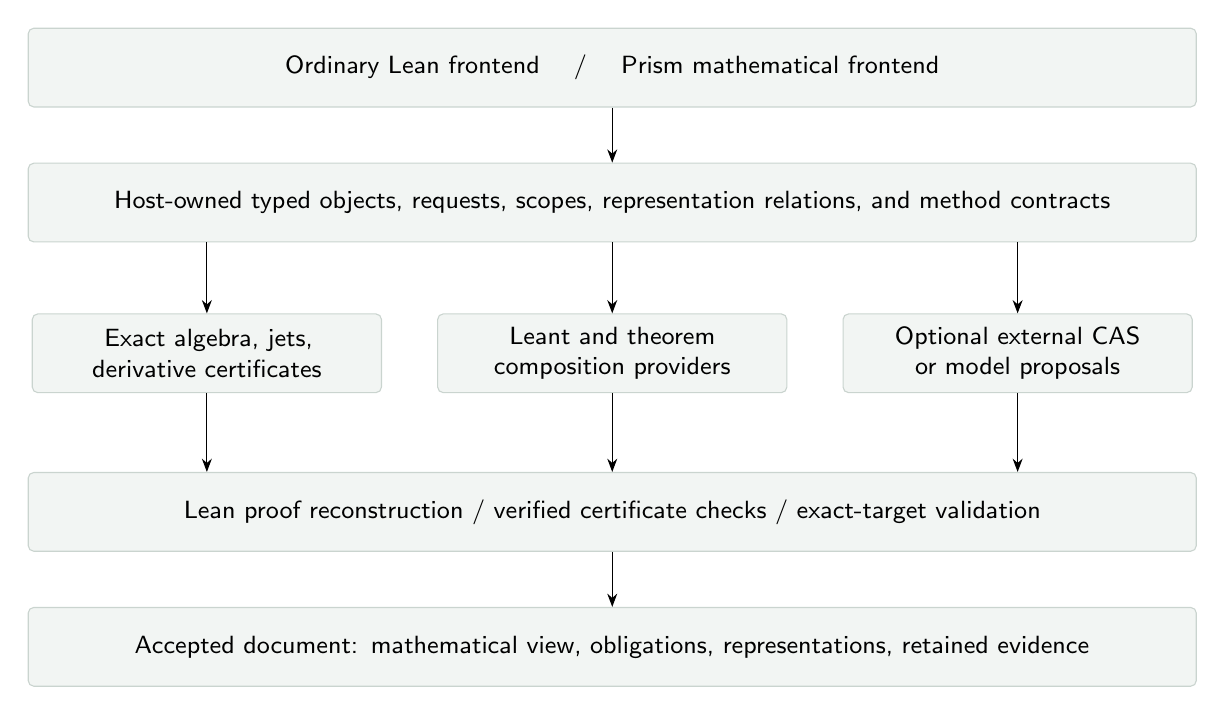
\begin{tikzpicture}[font=\small\sffamily,>=Stealth,
 box/.style={draw=rulegray,fill=panel,rounded corners=2pt,align=center,minimum height=10mm,text width=42mm},
 wide/.style={box,text width=146mm}]
\node[wide] (source) {Ordinary Lean frontend \quad / \quad Prism mathematical frontend};
\node[wide,below=7mm of source] (host) {Host-owned typed objects, requests, scopes, representation relations, and method contracts};
\node[box,below=9mm of host] (leant) {Leant and theorem\\composition providers};
\node[box,left=7mm of leant] (cas) {Exact algebra, jets,\\derivative certificates};
\node[box,right=7mm of leant] (external) {Optional external CAS\\or model proposals};
\node[wide,below=10mm of leant] (check) {Lean proof reconstruction / verified certificate checks / exact-target validation};
\node[wide,below=7mm of check] (artifact) {Accepted document: mathematical view, obligations, representations, retained evidence};
\draw[->] (source)--(host);
\draw[->] (host.south)--(leant.north);
\draw[->] (host.south -| cas.north)--(cas.north);
\draw[->] (host.south -| external.north)--(external.north);
\draw[->] (cas.south)--(check.north -| cas.south);
\draw[->] (leant.south)--(check.north);
\draw[->] (external.south)--(check.north -| external.south);
\draw[->] (check)--(artifact);
\end{tikzpicture}
\caption{One host-owned meaning boundary, several replaceable producers. Arrows from producers carry proposals and evidence to be checked, not assertions that the host must trust.}
\label{fig:architecture}
\end{figure}

The host owns the meaning of requests, scope, and acceptance. Domain packages own mathematical interfaces and certificate schemes. Providers own search strategies. Frontends own authoring and rendering. This ownership split is more important than whether the process boundary is Haskell-to-Lean, a local executable, or a plugin API.

\subsection{Milestones with observable gates}
\begin{enumerate}
\item \textbf{One certified value.} Implement polynomial-result requests with an exact denotation claim, source location, and a checked normalizer or certificate. Expose them in ordinary Lean first. Gate: accepted and deliberately corrupted outputs behave correctly, including an unsupported atom and a changed coefficient domain.
\item \textbf{One mixed mathematical proof.} Build the local derivative wrapper and the parameterized symbolic step behind the Lambert recurrence. Gate: the universal theorem replays with the producer unavailable; removing $W(x)\ne-1$ cannot silently retain the same derivative claim, and point equality cannot substitute for neighborhood equality.
\item \textbf{One definition interface.} Package EGF coordinates over a commutative $\Q$-algebra, including product and coefficient laws, plus finite-jet precision rules. Gate: the Abel coefficient theorem retains its arbitrary solution and coefficient-algebra generality; the derivative precision counterexample is rejected.
\item \textbf{The second frontend.} Add structured Prism steps and rendered mathematical notation over the same nodes. Gate: identical statements and interfaces are available in both frontends, and the source map explains every displayed mathematical claim.
\item \textbf{Leant integration.} Add the exact-context adapter, separate suggestion receipts, and whole-request budgets. Gate: replacing Leant with another proposal generator cannot change acceptance, and failed search never becomes a proof of nonexistence.
\item \textbf{Replay and representation maintenance.} Add dependency-aware replay, route metadata, and semantic edit classification. Gate: a provider can be removed without invalidating retained evidence in the pinned environment; a changed instance or object cannot reuse stale evidence unnoticed.
\end{enumerate}
These gates are proposed acceptance tests, not completed milestones. Hardening for arbitrary external code can proceed when deployment requires it; it should not replace the mathematical experiment.

\subsection{What should not be built first}
Do not begin with a natural-language parser, a global search over all possible representation routes, a general-purpose symbolic integration system, or a new kernel. Do not rewrite Leant's engines solely to make the architecture look uniform. Do not make a custom archive format more important than generated ordinary Lean that the user can inspect and maintain.

A verified sparse algebra substrate and a few well-designed interfaces can answer the central question. If even the Lambert and Abel examples cannot be expressed with predictable reconstruction and useful diagnostics, adding many more verbs will not fix the design.

\section{Evaluation: separate the language from the library}\label{sec:evaluation}
\subsection{The comparison that matters}
Use original Lean as a historical baseline, but use \emph{refactored Lean with the same interfaces} as the decisive baseline. Compare both frontends under the same deterministic methods; then enable the same Leant/CAS providers in each. Separately ablate the new definition packages to measure their contribution.

The experimental units should include at least the three inspected mathematical families, a numerical enclosure, and already-short proofs. Hold the theorem statement, coefficient structure, source environment, and allowed helper inventory fixed. A provider must not retrieve the target theorem, an alias of it, or downstream results that already contain its proof. A one-off helper equivalent to the target is not free infrastructure: count its authorship and proof cost.

\subsection{Measure work and explanation, not a single compression ratio}
Report author edits, time to a first accepted proof, time spent diagnosing failed operations, amount of explicit mathematical choice, generated obligation counts by role, producer and checker costs, retained evidence size, and repair work after controlled changes. Count interface development separately and amortize it across the actual evaluation suite.

Reader tasks should ask concrete questions: Which hypothesis licenses differentiation? Which endpoint is included in the reindexing? Does the theorem assume a field? Is this number exact or enclosed? Does the proposed solution list have a coverage proof? Which object changed after repair? These tasks are more informative than asking whether a language ``looks natural.''

A syntax-level compression ratio can be reported, but only alongside these costs. There is no reason to reward a one-word command whose hidden implementation contains the entire original proof and cannot be reused.

\subsection{Maintenance tests are part of the specification}
Perturb a theorem's wrapper mapping, rename an upstream binder, change a notation profile, replace a coefficient representation, increase requested jet precision, alter a branch domain, and remove an external provider. For each mutation, record which claims are reused, rechecked, or invalidated and whether the displayed explanation remains accurate.

Profile conflicts and multiple representation routes should be tested with two independently authored packages, not only with one designer's conventions. The correct behavior is either a certified coherent observation or an explicit conflict, not a silent route chosen because it happens to make the proof succeed.

\subsection{Stopping rules}
If representation packages and the ledger help but the new input syntax does not, ship the packages and reading view. If Leant does not improve composition beyond existing tactics on the chosen corpus, leave the adapter optional. If a certificate is too costly to check, keep the provider as a discovery assistant while developing a better certificate scheme. If a broad CAS operation repeatedly changes meanings or hides major hypotheses, narrow its contract.

These are useful outcomes. The goal is a better mathematical workflow, not preserving every component of a speculative design.

\section{What was actually checked for this article}\label{sec:experiments}
\subsection{The companion is an arithmetic model, not a proof assistant}
The included \code{experiments/exact_experiments.py} uses Python's standard-library exact rational arithmetic. It has no external dependencies. Its candidate producer and polynomial identity check are separately written, but neither the Python program nor Python's arithmetic implementation has been formally verified here. The results therefore provide reproducible finite tests and useful counterexamples, not kernel certificates.

\begin{center}\small
\begin{tabularx}{\textwidth}{@{}Y r@{}}
\toprule
Reported experiment & Checks\\
\midrule
Cross-multiplied Lambert derivative steps, $n=1,\ldots,8$ & 8\\
Corrupted Lambert candidates and invalid-index control rejected & 9\\
Binomial orthogonality for $0\le n,j<25$ & 625\\
Binomial orthogonality modulo $4,6,8$, for $0\le n,j<16$ & 768\\
EGF product coefficients over $\Q[\epsilon]/(\epsilon^2)$ & 520\\
EGF coordinate round trips over the same algebra & 520\\
Derivative precision counterexamples $t^N$, $1\le N\le20$ & 20\\
Exact endpoint signs for the root enclosure & 2\\
Truncated subtraction, natural division, and missing-pole-guard controls & 3\\
\midrule
Total reported checks, all passing their expected outcomes & 2,475\\
\bottomrule
\end{tabularx}
\end{center}
The dual-number tests use 40 deterministically seeded pairs of sequences through degree 12. The nonzero element $\epsilon$ satisfies $\epsilon^2=0$, so this explicitly exercises a rational algebra that is not a field. It does not replace the general proof of Proposition~\ref{prop:egf}.

The JSON receipt records the seed, scope, counts, and negative limitations. The certificate file records polynomial coefficient arrays and the exact rational enclosure. Running the program regenerates both files. These are deliberately small artifacts whose claims can be inspected without trusting a large experimental harness.

\subsection{Claims that remain unmeasured or unformalized}
No claim is made about Prism authoring speed, reader comprehension, proof-term size, Lean-checking latency, full-corpus migration rate, or Leant improvement. The new representation and precision theorems are proved on paper in this article but not formalized and checked in Lean here. The source inspection does not certify the repositories' build status.

The absence of those measurements is not a reason to avoid a concrete proposal. It is a reason to make its first executable gates specific and falsifiable. The article supplies a design that can be implemented incrementally, mathematical contracts whose edge cases are exposed, and an experiment that distinguishes those finite checks from the larger untested system.

\section{Conclusion: a language for changing form without changing mathematics}
A mathematician often suppresses details because an operation has a stable meaning in the current context: compare coefficients, differentiate a local identity, reindex a finite sum, normalize rational scalars, or bracket a uniquely specified root. A concise formal language should capture those operations and their scope, rather than merely hide arbitrary tactic scripts.

The first Brainstorm iteration already identified the right proof-assistant boundary. Prism extends it toward a mathematical workbench. Its central object is an accepted mathematical entity with certified representations; its central action is a computation returning an exact typed relationship; its central discipline is that guards, domains, precision, and solution coverage compose along with the computation.

The resulting hybrid is neither a conventional CAS with a proof checker bolted onto its output nor a proof assistant with an unrestricted ``ask CAS'' tactic. It is one typed document in which symbolic algorithms, ordinary theorem applications, finite computation, local analytic reasoning, and synthesis can exchange checked claims.

The recommended first investment is therefore concrete: a small polynomial-certificate interface, the local derivative-family example, and an EGF/jet representation package, exposed through both ordinary Lean and a mathematical frontend. Build the shared mathematical infrastructure first, keep the meaning boundary stable, and let measured authoring and reading results determine how much new language is worth retaining.

\appendix
\section{Decisions responding to the syntheses' open questions}\label{app:questions}
This crosswalk groups the questions in the final sections of the two syntheses rather than treating their formulations as votes. The answers below are design decisions or proposed experiments, not completed empirical findings.
\begin{longtable}{@{}P{.30\textwidth}P{.62\textwidth}@{}}
\toprule
Question family & Prism's answer and decision criterion\\
\midrule
\endhead
Document view or input language? & Both use one typed artifact. Compare the two frontends with identical methods; retain only a reading view if authoring does not improve. Sections~\ref{sec:surface}, \ref{sec:evaluation}.\\
Smallest useful method unit? & A stable theorem-wrapper schema, a computation certificate scheme, or a structural eliminator. Avoid one custom engine per verb. Section~\ref{sec:methods}.\\
Where does analysis plumbing live? & In a local-identity/derivative wrapper with exact neighborhood and derivative-existence premises; symbolic differentiation is a separate provider. Section~\ref{sec:lambert}.\\
How do views compose? & Ordered dependent guards and explicit relation composition. Anchor representations to the same semantic object; exact observation coherence resolves many diamonds without global normal forms. Sections~\ref{sec:rep}, \ref{sec:composition}.\\
How do roles survive refactoring? & Project-level semantic role IDs mapped to checked wrapper parameters. Upstream changes must rebuild that mapping; neither positions nor names are sufficient alone. Section~\ref{sec:methods}.\\
Which choices can be automatic? & Proof evidence, certified representation refinements, and explicitly delegated witness specifications. Freeze accepted objects; show plan and semantic changes. Sections~\ref{sec:result}, \ref{sec:methods}.\\
What is an honest provider verdict? & Checkable positive or negative evidence at a specified claim; otherwise conditional, unsupported, exhausted, cancelled, or rejected. Abstraction metadata is not an adequacy proof. Sections~\ref{sec:composition}, \ref{sec:leant}.\\
Is the Leant adapter worth building? & Measure composition separately from one-lemma retrieval, in both frontends. The adapter remains optional if existing tactics do as well. Sections~\ref{sec:leant}, \ref{sec:evaluation}.\\
What does a published data hole retain? & The selected object and its specification proof. Alternatives are optional exploration history, not necessary proof dependencies. Section~\ref{sec:methods}.\\
How strong is method conformance? & An explicit checked method tree for constrained steps; unrestricted permitted proof search for open checkpoints. No claim of premise indispensability. Section~\ref{sec:ui}.\\
Where does the definition layer start? & Interfaces for EGF coordinates, finite families, and certified constructions, not a general English parser. Count downstream bridge reductions and package cost. Sections~\ref{sec:egf}, \ref{sec:methods}.\\
What is the unit of replay? & A typed assertion or computation node with generated Lean and retained evidence. Distinguish source replay, certificate replay, and term replay. Section~\ref{sec:replay}.\\
How are notices dismissed? & Notices disclose resolved semantics and can be acknowledged per statement or explicit lexical profile. Acknowledgment never discharges an operation guard. See also Appendix~\ref{app:negative}.\\
Who owns conflicting policies? & Interpretation conflicts require selection; search providers can combine under explicit restrictions and budgets. Mathematical interfaces and operational policies version separately. Sections~\ref{sec:methods}, \ref{sec:ui}.\\
What is the stopping rule? & A useful Lean library, certificate API, or document renderer is sufficient. New syntax and providers must earn their place independently. Section~\ref{sec:evaluation}.\\
\bottomrule
\end{longtable}

\Needspace{32\baselineskip}
\section{A small surface grammar}\label{app:grammar}
This grammar sketches the structured layer. A prototype should embed Lean's term parser at \code{term}; the more mathematical ASCII notation used in worked examples is a presentation of the intended semantics, not an implemented parser specification. Declaration names and references resolve to stable host identities.
\begin{lstlisting}
document     ::= declaration*
declaration  ::= leanDeclaration | objectDecl | claimDecl | contextBlock
contextBlock ::= "context" profile* "{" declaration* "}"
objectDecl   ::= "define" name ":=" term
               | "construct" name ":" term "satisfying" term proof
claimDecl    ::= "claim" name? ":" term proof
proof        ::= "by" methodCall | "proof" "{" step* "}"
step         ::= "assume" binder
               | "obtain" pattern "from" term
               | claimDecl
               | "compute" name ":=" request
               | "work" "in" representation "of" term
               | "calc" relationChain
               | "cases" term branch*
               | "induct" binder "with invariant" term branch*
               | "conclude" term? "by" methodCall
               | "lean" "{" leanTactics "}"
request      ::= operation term* ("on" term)? ("to precision" term)?
                 ("in form" term)? ("using" dependencyPolicy)?
methodCall   ::= methodName argument* | "search" searchPolicy
relationChain::= (term relation term "by" methodCall)+
\end{lstlisting}
The grammar intentionally has no operation meaning ``silently strengthen the theorem until it is provable.'' A suggestion can propose such a statement edit, but it is a different declaration requiring explicit acceptance.

\section{Negative neighbors for the first implementation}\label{app:negative}
Each positive domain example should ship with a neighboring failure. The expected outcome includes a specific missing or false claim, not merely a red status on the whole proof.
\begin{longtable}{@{}P{.06\textwidth}P{.43\textwidth}P{.43\textwidth}@{}}
\toprule
ID & Mutation & Required behavior\\
\midrule
\endhead
N1 & Reindex $[j,n]$ by $j+i$ with $0\le i<m$. & Reject coverage of $n$; do not keep the claimed method while proving the target another way.\\
N2 & Transport $(2-3:\N)$ as integer subtraction. & Require the missing order guard or preserve truncated subtraction.\\
N3 & Transport natural division $1/2$ as rational division. & Require exactness/divisibility or state the changed expression.\\
N4 & Cancel $x-1$ at $x=1$. & Keep the conditional result, split cases, or return a checked piecewise expression.\\
N5 & Multiply a strict inequality by a merely nonnegative factor. & Require strict positivity or handle the zero case explicitly.\\
N6 & Differentiate $f(0)=g(0)$ for $f(t)=t$, $g(t)=0$. & Reject local-equality transfer: the values agree but derivatives do not.\\
N7 & Use the Lambert rational derivative form at $w=-1$. & Retain the excluded-point obligation; a total expression value does not supply the derivative theorem.\\
N8 & Differentiate a precision-$N$ jet as though it retained precision $N$. & Reject using $t^N$ versus zero over $\Q$; demand one more coefficient.\\
N9 & Read a finite formal expansion as an analytic estimate. & Require a convergence/remainder bridge, not just matching coefficients.\\
N10 & Read validated root candidates as a complete root list. & Require solution coverage, with the chosen domain and multiplicities where requested.\\
N11 & Prove a radical identity by equality of squares alone. & Require sign/branch evidence or retain both branches.\\
N12 & Strengthen the Abel coefficient ring to a field. & Classify as a statement change, not an implementation repair.\\
N13 & Replace an arbitrary solution $T$ by the canonical Abel series. & Require an equality/uniqueness bridge or preserve the arbitrary $T$.\\
N14 & Reuse a candidate from a sibling branch or prior worker generation. & Reject the scope or origin mismatch before acceptance.\\
N15 & Exhaust a search and report the theorem false. & Return exhaustion unless an original-claim negation certificate is checked.\\
N16 & Include a false but unused intermediate assertion. & Reject the document even if its final theorem is otherwise proved.\\
N17 & Acknowledge a notice about total division. & Record the convention only; do not discharge any nonzero guard.\\
N18 & Change an algebra instance with unchanged displayed notation. & Invalidate the semantic request and show the instance-level change.\\
N19 & Accept suggested source text that differs from the tested tactic. & Reapply the exact displayed patch from its recorded starting state.\\
N20 & Submit an unapproved axiom through a dependency. & Reject publication under the chosen transitive axiom policy.\\
\bottomrule
\end{longtable}
These are specification cases. Only the limited arithmetic subset described in Section~\ref{sec:experiments} was executed for this article.

\section{Source and artifact notes}\label{app:source}
The accompanying \code{evidence/source-register.json} records the inspected repository revisions and files. The bibliography links to commit-pinned repository sources wherever possible. Public documentation links are separately identified as moving references consulted during preparation; they do not assert compatibility with an uninspected project toolchain.

The repository timestamps for some inspected commits fall on 6 September in UTC but on 5 September in Pacific time. The article's date uses the latter. No unpublished local working tree described in a source report is claimed to have been reproduced here.

The ZIP contains this self-contained \LaTeX{} source and its rendered PDF, a build/readme file, the exact-arithmetic script and its outputs, and the source register. No external figures, proprietary font files, or original repository archives are required to rebuild the article. Standard \TeX{} Live packages suffice.

\begin{thebibliography}{99}
\small
\bibitem{synA} Brainstorm project.
\emph{Mathematical Ideas, Checked Evidence}.
\code{docs/synthesis/unified-report.tex}, inspected at commit
\code{494be9d5ab41a5ae219fc6f800e6aee3c93bce39}.
\url{https://github.com/VladimirReshetnikov/Brainstorm/blob/494be9d5ab41a5ae219fc6f800e6aee3c93bce39/docs/synthesis/unified-report.tex}.

\bibitem{synB} Claude (Anthropic), for Vladimir Reshetnikov.
\emph{Nine Blueprints for a Mathematician's Proof Language over Lean}.
\code{docs/unified_report/unified_report.tex}, same Brainstorm revision.
\url{https://github.com/VladimirReshetnikov/Brainstorm/blob/494be9d5ab41a5ae219fc6f800e6aee3c93bce39/docs/unified_report/unified_report.tex}.

\bibitem{binomial} ProveIt project.
\emph{BinomialInversion.lean}.
Commit \code{24ce8bd743eaab64a91ce90725ea00f498d319d2}.
\url{https://github.com/VladimirReshetnikov/ProveIt/blob/24ce8bd743eaab64a91ce90725ea00f498d319d2/Analysis/FabiusFunction/Lean/FabiusFunction/BinomialInversion.lean}.

\bibitem{ode} ProveIt project.
\emph{AutonomousIteratedDeriv.lean}. Same ProveIt revision.
\url{https://github.com/VladimirReshetnikov/ProveIt/blob/24ce8bd743eaab64a91ce90725ea00f498d319d2/Analysis/FabiusFunction/Lean/FabiusFunction/AutonomousIteratedDeriv.lean}.

\bibitem{abel} ProveIt project.
\emph{AbelPolynomialSeries.lean}. Same ProveIt revision.
\url{https://github.com/VladimirReshetnikov/ProveIt/blob/24ce8bd743eaab64a91ce90725ea00f498d319d2/Analysis/FabiusFunction/Lean/FabiusFunction/AbelPolynomialSeries.lean}.

\bibitem{verification} Leant project.
\emph{src/Leant/Synth/Verification.hs}.\par
Commit \code{3a40904be8a410d832d9ab6900b3d3e7b425eccb}.
\url{https://github.com/VladimirReshetnikov/Leant/blob/3a40904be8a410d832d9ab6900b3d3e7b425eccb/src/Leant/Synth/Verification.hs}.

\bibitem{engine} Leant project.
\emph{src/Leant/Synth/Engine.hs}. Same Leant revision.
Engine boundary, outcome types, and exact candidate provenance.
\url{https://github.com/VladimirReshetnikov/Leant/blob/3a40904be8a410d832d9ab6900b3d3e7b425eccb/src/Leant/Synth/Engine.hs}.

\bibitem{main} Leant project.
\emph{src/Main.hs}. Same Leant revision.
Selected suggestion/probe code, including \code{probeOnce} and \code{parseTryThis} use.
\url{https://github.com/VladimirReshetnikov/Leant/blob/3a40904be8a410d832d9ab6900b3d3e7b425eccb/src/Main.hs}.

\bibitem{harrison} John Harrison and Laurent Th\'ery.
``A Skeptic's Approach to Combining HOL and Maple.''
\emph{Journal of Automated Reasoning} 21 (1998), 279--294.
Author's publication page and abstract:
\url{https://www.cl.cam.ac.uk/~jrh13/papers/cas.html}.

\bibitem{transfer} Isabelle project.
\emph{Isar Reference Manual: HOL-Specific Tools}, Lifting and Transfer sections.
Official online reference consulted 5 September 2026.
\url{https://isabelle.in.tum.de/dist/library/Doc/Isar_Ref/HOL_Specific.html}.

\bibitem{leanvalidation} Lean project.
\emph{The Lean Language Reference: Validating a Lean Proof}.
Moving online reference consulted 5 September 2026; in particular its distinction between statement meaning and proof checking, and its native-evaluation discussion.
\url{https://lean-lang.org/doc/reference/latest/ValidatingProofs/}.

\bibitem{ring} Mathlib project.
\emph{Mathlib.Tactic.Ring.Basic}.
Online API documentation consulted 5 September 2026.
\url{https://leanprover-community.github.io/mathlib4_docs/Mathlib/Tactic/Ring/Basic.html}.

\bibitem{polyrith} Mathlib project.
\emph{Mathlib.Tactic.Polyrith}.
Online documentation consulted 5 September 2026; its current deprecation notice distinguishes the historical tactic from the supported alternatives.
\url{https://leanprover-community.github.io/mathlib4_docs/Mathlib/Tactic/Polyrith.html}.

\bibitem{interval} Guillaume Melquiond and contributors.
\emph{Interval Package for Rocq}.
Official overview and documentation consulted 5 September 2026.
\url{https://coqinterval.gitlabpages.inria.fr/}.

\bibitem{afp} Manuel Eberl and Ren\'e Thiemann.
\emph{Factorization of Polynomials with Algebraic Coefficients}.
Archive of Formal Proofs, 2021. Entry and linked formal theories.
\url{https://isa-afp.org/entries/Factor_Algebraic_Polynomial.html}.

\bibitem{egg} Marcus Rossel and contributors.
\emph{lean-egg: Equality Saturation Tactic for Lean}.
Project status and documentation consulted 5 September 2026; the repository marks the tactic deprecated and recommends \code{grind}.
\url{https://github.com/marcusrossel/lean-egg}.
\end{thebibliography}
\end{document}
